%%%%%%%%%%%%%%%%%%%%%%%%%%%%%%%%%%%
%This is the LaTeX ARTICLE template for RSC journals
%Copyright The Royal Society of Chemistry 2016
%%%%%%%%%%%%%%%%%%%%%%%%%%%%%%%%%%%

\documentclass[twoside,twocolumn,9pt]{article}

\usepackage{tgheros}
\renewcommand{\familydefault}{\sfdefault}

\usepackage{extsizes}
\usepackage[super,sort&compress,comma]{natbib} 
\usepackage[version=3]{mhchem}
\usepackage[left=1.5cm, right=1.5cm, top=1.785cm, bottom=2.0cm]{geometry}
\usepackage{balance}
\usepackage{mathptmx}
\usepackage{sectsty}
\usepackage{graphicx} 
\usepackage{lastpage}
\usepackage[format=plain,justification=justified,singlelinecheck=false,font={stretch=1.125,small,sf},labelfont=bf,labelsep=space]{caption}
\usepackage{float}
\usepackage{fancyhdr}
\usepackage{fnpos}
\usepackage[english]{babel}
\addto{\captionsenglish}{%
  \renewcommand{\refname}{Notes and references}
}
\usepackage{array}
\usepackage{droidsans}
\usepackage{charter}
\usepackage[T1]{fontenc}
\usepackage[usenames,dvipsnames]{xcolor}
\usepackage{setspace}
\usepackage[compact]{titlesec}
%%%Please don't disable any packages in the preamble, as this may cause the template to display incorrectly.%%%


\usepackage{xcolor}
\definecolor{ugent_blue}{RGB}{30, 100, 200}
\definecolor{ugent_yellow}{cmyk}{.0, .10, 1, 0}

\usepackage{titlesec}
\titleformat{\section}
{\color{ugent_blue}\normalfont\Large\bfseries}
{\color{ugent_blue}\thesection}{1em}{}

\usepackage[colorlinks=true,linkcolor=black,citecolor=ugent_blue]{hyperref}

%\AtEveryCite{\color{ugent_blue}}
\usepackage{parskip}
\usepackage{epstopdf}%This line makes .eps figures into .pdf - please comment out if not required.
\usepackage{cleveref}
\definecolor{cream}{RGB}{222,217,201}

\begin{document}

\pagestyle{fancy}
\thispagestyle{plain}
\fancypagestyle{plain}{
%%%HEADER%%%
\renewcommand{\headrulewidth}{0pt}
}
%%%END OF HEADER%%%

%%%PAGE SETUP - Please do not change any commands within this section%%%
\makeFNbottom
\makeatletter
\renewcommand\LARGE{\@setfontsize\LARGE{15pt}{17}}
\renewcommand\Large{\@setfontsize\Large{12pt}{14}}
\renewcommand\large{\@setfontsize\large{10pt}{12}}
\renewcommand\footnotesize{\@setfontsize\footnotesize{7pt}{10}}
\makeatother

\renewcommand{\thefootnote}{\fnsymbol{footnote}}
\renewcommand\footnoterule{\vspace*{1pt}% 
\color{cream}\hrule width 3.5in height 0.4pt \color{black}\vspace*{5pt}} 
\setcounter{secnumdepth}{5}

\makeatletter 
\renewcommand\@biblabel[1]{#1}            
\renewcommand\@makefntext[1]% 
{\noindent\makebox[0pt][r]{\@thefnmark\,}#1}
\makeatother 
\renewcommand{\figurename}{\small{Fig.}~}
\sectionfont{\sffamily\Large}
\subsectionfont{\normalsize}
\subsubsectionfont{\bf}
\setstretch{1.125} %In particular, please do not alter this line.
\setlength{\skip\footins}{0.8cm}
\setlength{\footnotesep}{0.25cm}
\setlength{\jot}{10pt}
\titlespacing*{\section}{0pt}{4pt}{4pt}
\titlespacing*{\subsection}{0pt}{15pt}{1pt}
%%%END OF PAGE SETUP%%%

%%%FOOTER%%%
\fancyfoot{}
\fancyfoot[LO,RE]{\vspace{-7.1pt}
\includegraphics[height=9pt]{head_foot/LF}}
\fancyfoot[CO]{\vspace{-7.1pt}\hspace{11.9cm}
\includegraphics{head_foot/RF}}
\fancyfoot[CE]{\vspace{-7.2pt}\hspace{-13.2cm}
\includegraphics{head_foot/RF}}
\fancyfoot[RO]{\footnotesize{\sffamily{1--\pageref{LastPage} {\color{ugent_yellow} ~\textbar } \hspace{2pt}\thepage}}}
\fancyfoot[LE]{\footnotesize{\sffamily{\thepage~{\color{ugent_yellow} ~\textbar }\hspace{4.65cm} 1--\pageref{LastPage}}}}
\fancyhead{}
\renewcommand{\headrulewidth}{0pt} 
\renewcommand{\footrulewidth}{0pt}
\setlength{\arrayrulewidth}{1pt}
\setlength{\columnsep}{6.5mm}
\setlength\bibsep{1pt}
%%%END OF FOOTER%%%

%%%FIGURE SETUP - please do not change any commands within this section%%%
\makeatletter 
\newlength{\figrulesep} 
\setlength{\figrulesep}{0.5\textfloatsep} 

\newcommand{\topfigrule}{\vspace*{-1pt}% 
\noindent{\color{cream}\rule[-\figrulesep]{\columnwidth}{1.5pt}} }

\newcommand{\botfigrule}{\vspace*{-2pt}% 
\noindent{\color{cream}\rule[\figrulesep]{\columnwidth}{1.5pt}} }

\newcommand{\dblfigrule}{\vspace*{-1pt}% 
\noindent{\color{cream}\rule[-\figrulesep]{\textwidth}{1.5pt}} }

\makeatother
%%%END OF FIGURE SETUP%%%

%%%TITLE, AUTHORS AND ABSTRACT%%%
\twocolumn[
  \begin{@twocolumnfalse}
{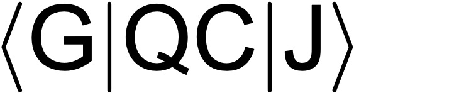
\includegraphics[height=30pt]{head_foot/journal_name}\hfill\raisebox{0pt}[0pt][0pt]{
\includegraphics[height=55pt]{head_foot/RSC_LOGO_CMYK}}\\[1ex]

\includegraphics[width=18.5cm]{head_foot/header_bar}}\par
\vspace{1em}
\sffamily
\begin{tabular}{m{4.5cm} p{13.5cm} }

& \noindent\LARGE{\textbf{Characterization of reactions in the Huckel model using fluctuations and entanglement$^\dag$}} \\%Article title goes here instead of the text "This is the title"
\vspace{0.3cm} & \vspace{0.3cm} \\

& \noindent\large{Mattice Criel$^{b}$, Ruben Van der Stichelen$^{a}$, Daria Van Hende$^{a}$, Xeno De Vriendt$^{a}$, Patrick Bultinck$^{a}$ and Guillaume Acke$^{a}$} \\%Author names go here instead of "Full name", etc.

& \\

& \noindent\normalsize{In this study, we use the H$\ddot{\text{u}}$ckel Molecular Orbital (HMO) model and quantum information measures to analyze the $\pi$-system of benzene and its response to the introduction of a chemical potential, serving as a proxy for introducing a hetero atom. When interactions between specific carbon atoms are reduced to zero, mimicking transitions to different molecular structures like hexa-1,3,5-triene, an alternated electron distribution pattern emerges. Furthermore, we find that the position of a manipulated carbon atom influences the extent of electron redistribution and entanglement within the system. At the end, we will also show how the HMO model with applied chemical potential can be linked to organic chemistry and how it can be used to get insight in the reactivity of substituted conjugated systems. Our findings provide insight into using the chemical potential in HMO and into the role of quantum measurements in understanding the behavior of conjugated $\pi$-systems under different conditions.} \\%The abstrast goes here instead of the text "The abstract should be..."

\end{tabular}

\end{@twocolumnfalse} \vspace{1.6cm}

  ]
%%%END OF TITLE, AUTHORS AND ABSTRACT%%%

%%%FONT SETUP - please do not change any commands within this section
\renewcommand*\rmdefault{bch}\normalfont\upshape
\rmfamily
\section*{}
\vspace{-1cm}


% %%%FOOTNOTES%%%

\footnotetext{\textit{$^{a}$~Ghent Quantum Chemistry Group, Krijgslaan 281 (S3), B-9000 Gent, Belgi$\ddot{\text{e}}$}}
\footnotetext{\textit{$^{b}$~Corresponding author:} \texttt{Mattice.Criel@ugent.be}}

% %Please use \dag to cite the ESI in the main text of the article.
% %If you article does not have ESI please remove the the \dag symbol from the title and the footnotetext below.
% \footnotetext{\dag~Electronic Supplementary Information (ESI) available: [details of any supplementary information available should be included here]. See DOI: 00.0000/00000000.}
% %additional addresses can be cited as above using the lower-case letters, c, d, e... If all authors are from the same address, no letter is required

% \footnotetext{\ddag~Additional footnotes to the title and authors can be included \textit{e.g.}\ `Present address:' or `These authors contributed equally to this work' as above using the symbols: \ddag, \textsection, and \P. Please place the appropriate symbol next to the author's name and include a \texttt{\textbackslash footnotetext} entry in the the correct place in the list.}


%%%END OF FOOTNOTES%%%

%%%MAIN TEXT%%%%


\section{Introduction}
While modern ab initio quantum chemistry methods have surpassed simple models when it comes to quantitative descriptions of systems, such models still serve an important role in the current research climate. The H$\ddot{\text{u}}$ckel molecular orbital (HMO) model, for example, is often seen as an indispensable tool in the general understanding of conjugated $\pi$-systems and many organic chemistry textbooks use H$\ddot{\text{u}}$ckel based arguments whenever the conditions for their applicability are met \cite{kutzelnigg2007}. The strength of the HMO model lies in its purposely simplified approach to reality, which accounts only for certain aspects of reality, but does so in a convincing way.

The model restricts the attention to so-called \emph{covalent many-center bonds} and considers those aspects which are related to mobile
$\pi$-electrons. Since the $\sigma$-framework is usually localized and regarded as transferable between molecules, it is decoupled from
the $\pi$-framework and therefore not explicitly considered. Furthermore, only situations largely unaffected by bond formation of delocalization are taken into account, justifying a \emph{one-electron theory} \cite{kutzelnigg2007}. Since Coulomb interactions are inversely proportional to the distance between two charges, long-range interactions will hardly play any role which justifies the limitation to only \emph{nearest neighbor interactions} \cite{kutzelnigg2007}. This way, the H$\ddot{\text{u}}$ckel model is reduced to the topology of the system under study. Lastly, the overlap integral between the $2p_z$ atomic orbitals (AO) is assumed zero, which
renders the underlying basis set orthonormal.

The epitome of the HMO model is found in the treatment of the $\pi$-system of benzene. The description of alternant hydrocarbons, such as benzene, using the HMO model allows for the analytic determination of the molecular orbital (MO) energies as well as the corresponding AO coefficients of these MO's (\cref{fig:diagram benzene}) which are represented in terms of $\alpha$ and $\beta$, the Coulomb and resonance integrals respectively. The value of the parameters can be arbitrary chosen here.

  \begin{figure}[h]
  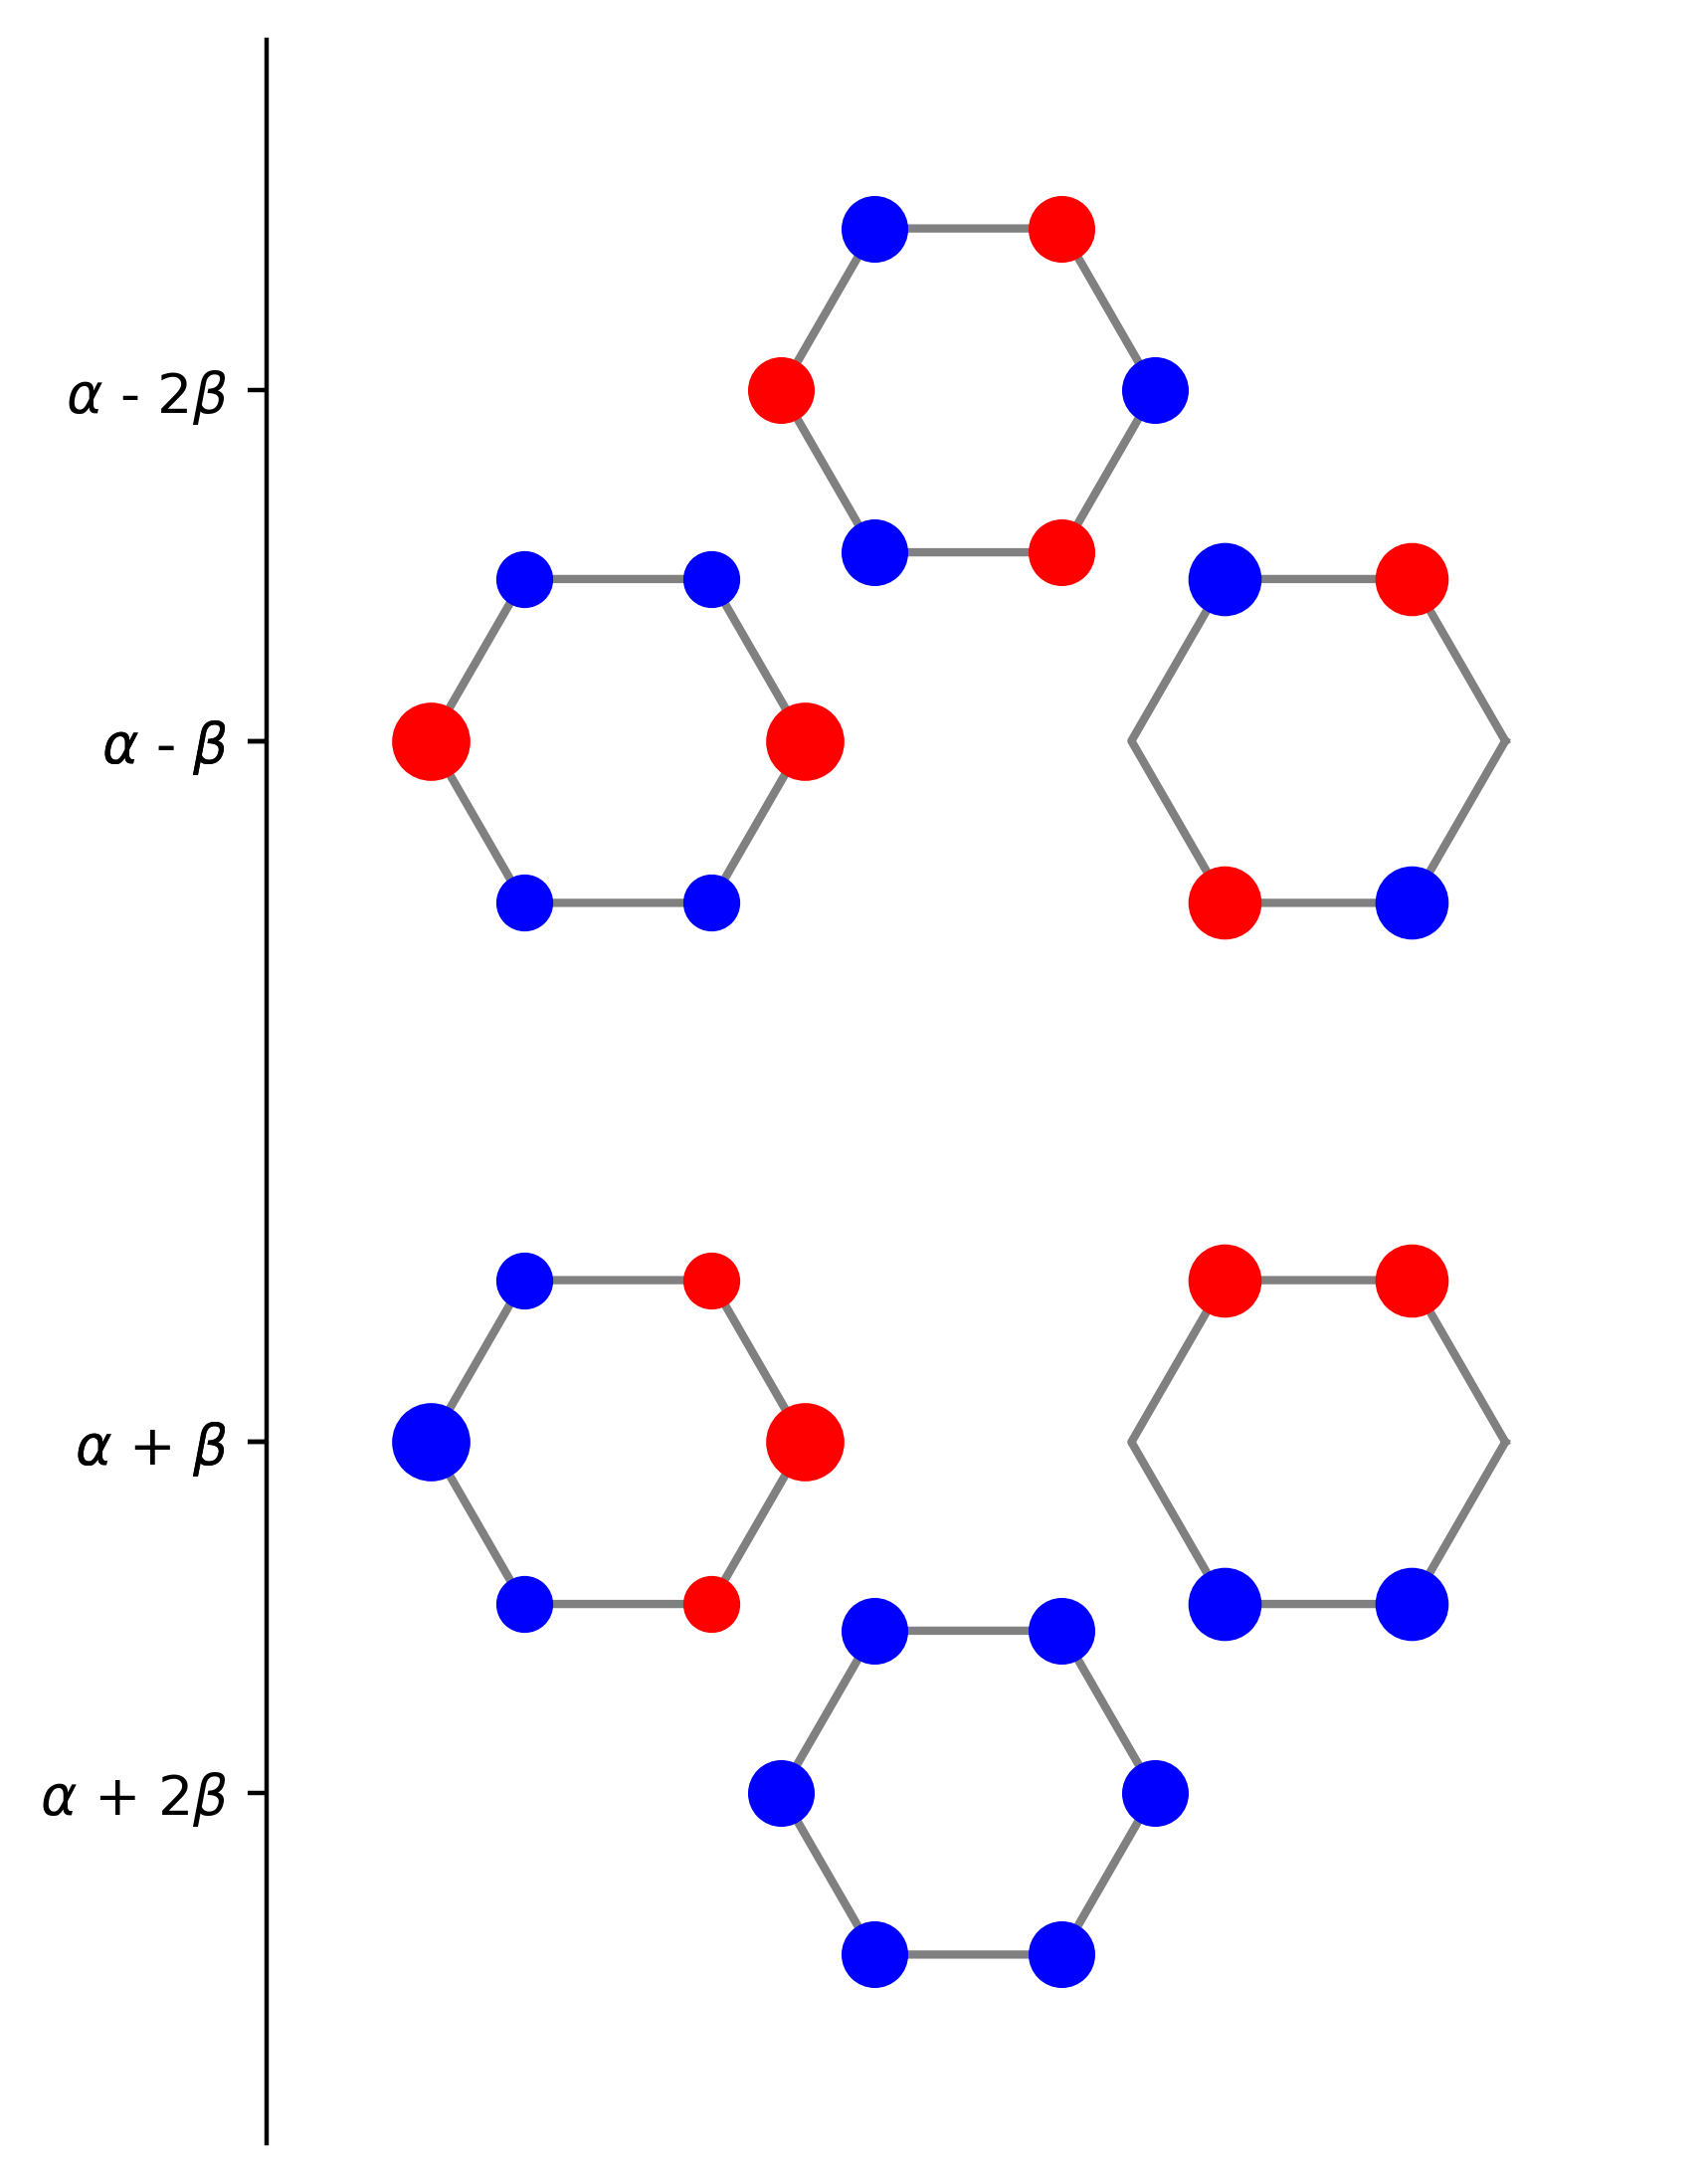
\includegraphics[width=\linewidth]{diagram_huckel_MO's.png}
  \caption{The 6 $\pi$ MO's for benzene obtained with the H$\ddot{\text{u}}$ckel model where the color and size of the dot represent the sign and value of the coefficient of the 2$p_z$ atomic orbitals, the corresponding orbital energies can be seen on the y-axis}
  \label{fig:diagram benzene}
  \end{figure}

  The H$\ddot{\text{u}}$ckel Molecular Orbital model can be justified for these conjugated $\pi$-systems because the same results are obtained for the $\pi$ molecular orbitals when they are calculated using Restricted Hartree-Fock (RHF) theory in the STO-3G basis set (\cref{sec:HMO vs RHF for benzene}). Although we see that the energies differ, this is not a problem because in this paper we are only working with the electronic structures of the orbitals which are equally described.

  % To justify the use of the H$\ddot{\text{u}}$ckel Molecular Orbital model for benzene, we compare its molecular orbitals (MO's) and corresponding energies with those calculated using Restricted Hartree-Fock (RHF) theory in the STO-3G basis set (\cref{sec:HMO vs RHF for benzene}). Both HMO and RHF predict a similar qualitative ordering of the molecular orbital energy levels and reflect the $D_{6h}$ symmetry of the benzene molecule, capturing the delocalized nature of the $\pi$-electrons over the benzene ring. However, a difference can be seen because RHF provides a more accurate quantitative description of orbital energies as it incorporates electron-electron repulsion more comprehensively, whereas HMO simplifies interactions significantly. The electronic structure of the $\pi$ molecular orbitals calculated with HMO and RHF are the same and only the $2p_z$ atomic orbitals attribute to the MO's in RHF which tells us that the approximation of using the $2p_z$ atomic orbitals as basis in HMO to describe the $\pi$-system is justified. In this work, we can ignore the difference between both because we will work only with the electronic structure which is equally described. 
% \begin{itemize}
%   \item Introduce $\alpha$ and $\beta$ based on the sentence above. 
%   \item Why can this Huckel model be seen as parameter free?
%   \item How can we prove the strength of this description from the Hückel model: compare to restricted Hartree-Fock.
%   \item What are the similarities with an ab-initio quantum chemistry method like RHF?
%   \item What are the differences with such a method?
%   \item Why can or can we not ignore these differences? 
%   \item Reference figure of RHF versus HMO molecular orbitals, but move figiure to appendix. 
% \end{itemize}
  % Despite entanglement measures being widely applied in condensed matter physics for large systems\cite{LAFLORENCIE20161}, their utilization in quantum chemistry remains relatively unexplored. The smaller molecules, used in numerous chemical processes and materials, offer a captivating landscape for exploring quantum phenomena such as entanglement, which proves to be valuable in the condensed matter physics for describing the correlation between different electronic domains.

Thus far, we have treated the HMO model as parameter free. However, to incorporate some neglected effects of electron-electron interaction the HMO model is often treated as a \emph{semi-empirical model} \cite{Pow}. For example, the $\alpha$ parameter can be modified based on the charge on the atom, introducing an additional form of Coulomb repulsion to the HMO model. Such parametrizations only slightly complicate the model but do not lead to major inflation of the computational cost and often greatly increase the accuracy of the predictions. Another way to expand on the HMO model arises from the case of the \emph{tight binding model} which is the terminology used when the H$\ddot{\text{u}}$ckel model is applied to systems where the number of particles approaches the thermodynamic limit. In these cases, keeping track of the particles becomes cumbersome. Lagrange's multipliers \cite{arfken1995mathematical}  are a powerful general method to impose constraints on differential equations without modifying the integro-differential equations and can constrain the electron population on a site. So, we are going to use a Lagrange multiplier in HMO by subtracting $\mu\hat{N}$ from the Hamiltonian to control the number of electrons on a site by the parameter $\mu$, the chemical potential.

% A Lagrange multiplier can be introduced to resolve the difficulty of constraining the number of electrons in the thermodynamic limit.
% By subtracting $\mu\hat{N}$ from the Hamiltonian we can control the number of electrons by the parameter $\mu$, the chemical potential.
% The introduction of a chemical potential can be viewed as a proxy for introducing a hetero atom into the system, as it allows us to simulate the effects of different chemical influences without explicitly modifying the atomic composition. This can help in studying the impact of electron-donating and electron-withdrawing groups on the electronic structure of the system. Furthermore, interactions ($\beta$) can also be constrained, which means we can analyze how a system changes when the interaction is broken.
% \begin{itemize}
%   \item Read section on chemical potential from Powell 2010. Shop there for a further explication. 
%   \item The introduction of a chemical potential can be viewed as a proxy of introducing a hetero atom into the system. \textbf{$\rightarrow$ WHY?}
%   \item Interactions ($\beta$) can also be \emph{constrained}, explain what this means as well. 
% \end{itemize}

In this work, we will use the Lagrange multiplier methodology to apply several such chemical potentials onto the $\pi$-system of benzene and observe how this affects the electronic structure of our system. When applying a Lagrange multiplier on the Coulomb integral, we can control the potential on an atom which will act as an electron donating group or electron withdrawing group. This can be seen as introducing a hetero atom into the system. We will further look at the limit of zero interaction for one or more of the resonance integrals by introducing a Lagrange multiplier that act on $\beta$ as a proxy of breaking bonds in the system. 

% \begin{itemize}
%   \item proxy of introducing a hetero atom into the system \textbf{$\rightarrow$ electron donating group versus electron withdrawing groups}
%   \item We will look  at the limit of zero interaction for one or more of the resonance integrals, Why do we do this?
%   \item What does the Lagrange constraint allow us to observe in this case?
% \end{itemize}

Quantum entanglement measures are on the rise in the field of quantum chemistry \cite{DeVriendt2022}$^,$\cite{Daria1}$^,$\cite{Pendas}$^,$\cite{tubman2014quantum} and are well-suited quantum probes to study the behavior of electrons in strongly correlated systems \cite{LAFLORENCIE20161}. Therefore, we will use quantum entanglement measures in order to examine the correlation pathways and how these are affected by the applied chemical potential.
  % In quantum chemistry, many conjugated $\pi$-systems have been investigated using the H$\ddot{\text{u}}$ckel Molecular Orbital (HMO) model, even modelling hetero atoms by adjusting various parameters. Additionally, Delocalization Indices have been applied to these systems\cite{C5CP06098B}. This suggests the potential for further extension of quantum measures, like using mutual information, to extract more comprehensive quantum information of conjugated systems.
  
  % We aim to analyze the $\pi$-system of benzene using the H$\ddot{\text{u}}$ckel Molecular Orbital model and observe its response to the introduction of a chemical potential. We will first establish that HMO is a good approximating for the $\pi$-system by comparing it with Restricted Hartree-Fock (RHF) calculations (figure \ref{fig:diagram benzene}). The introduction of a chemical potential can be viewed as a proxy of introducing a hetero atom into the system. Additionally, we will explore the effects on the electronic structure of reducing different interaction by examine the electron distribution and mutual information.

By reducing the interaction of one bond in benzene to zero, we approximate the structure of hexa-1,3,5-triene, revealing an alternated and conjugated $\pi$-system. This suggests that the introduction of a chemical potential will have a different influence on the electronic structure of the $\pi$-systems of benzene and hexa-1,3,5-triene. Furthermore, we demonstrate that the position of a chemical potential impacts the changes in the electronic structure. This is done by reducing two $\beta$ parameters to simulate a transition from benzene to a butadiene and ethene. By placing the carbon atom, on which we apply a chemical potential, in the approximated butadiene, we can demonstrate the different effects of placing the carbon atom as an outer or inner carbon atom.

% \begin{itemize}
%   \item This suggests that the introduction of a chemical potential will have a different influence on the electronic structure of both $\pi$ systems. \textbf{$\rightarrow$ HOW?}
%   \item Furthermore, we demonstrate that the position of a chemical potential impacts the changes in the electronic structure. \textbf{$\rightarrow$ HOW?}
%   \item We also reduce the interaction of two $\beta$ parameters $\rightarrow$ Why? What does this mean? 
% \end{itemize}
 
Our approach offers a novel perspective on understanding the entanglement of conjugated $\pi$-systems and the impact of introducing constraints on the Hamiltonian. By exploring these aspects, we further elucidate the strength of the H$\ddot{\text{u}}$ckel model when it comes to the description of these conjugated $\pi$-systems and expand upon the well-known chemical applicability of the model.


  % Despite entanglement measures being widely applied in condensed matter physics for large systems\cite{LAFLORENCIE20161}, their utilization in quantum chemistry remains relatively unexplored. The smaller molecules, used in numerous chemical processes and materials, offer a captivating landscape for exploring quantum phenomena such as entanglement, which proves to be valuable in the condensed matter physics for describing the correlation between different electronic domains.
  
  % In quantum chemistry, many conjugated $\pi$-systems have been investigated using the H$\ddot{\text{u}}$ckel Molecular Orbital (HMO) model, even modelling hetero atoms by adjusting various parameters. Additionally, Delocalization Indices have been applied to these systems\cite{C5CP06098B}. This suggests the potential for further extension of quantum measures, like using mutual information, to extract more comprehensive quantum information of conjugated systems.
  
  % We aim to analyze the $\pi$-system of benzene using the H$\ddot{\text{u}}$ckel Molecular Orbital model and observe its response to the introduction of a chemical potential. We will first establish that HMO is a good approximating for the $\pi$-system by comparing it with Restricted Hartree-Fock (RHF) calculations (figure \ref{fig:diagram benzene}). The introduction of a chemical potential can be viewed as a proxy of introducing a hetero atom into the system. Additionally, we will explore the effects on the electronic structure of reducing different interaction by examine the electron distribution and mutual information.

  % By reducing the interaction of one bond in benzene to zero, we approximate the structure of hexa-1,3,5-triene, revealing an alternated and conjugated $\pi$-system. This suggests that the introduction of a chemical potential will have a different influence on the electronic structure of both $\pi$ systems. Furthermore, we demonstrate that the position of a chemical potential impacts the changes in the electronic structure.
  
  % Our approach offers a novel perspective on understanding the entanglement of conjugated $\pi$-systems and the impact of introducing constraints on the Hamiltonian. By exploring these aspects, we contribute to advancing the understanding of quantum phenomena in chemical systems and pave the way for further research in this area.


\section{Theory}
\subsection{H$\ddot{\text{u}}$ckel Molecular Orbital model}

We introduce the matrix representation of the H$\ddot{\text{u}}$ckel Hamiltonian as follows
\begin{equation}
  h_{\text{H$\ddot{\text{u}}$ckel }} = \left\{
  \begin{aligned}
    & \langle \phi_i | \hat{h} | \phi_i \rangle = h_{ii} = \alpha\\
    & \langle \phi_i | \hat{h} | \phi_j \rangle = h_{ij} = h_{ji} = \beta \quad \text{if } i \text{ and } j \text{ are adjacent}\\
    & \langle \phi_i | \hat{h} | \phi_j \rangle = 0 \quad \text{if } i \text{ and } j \text{ are not adjacent}\\
  \end{aligned}
  \right.
\end{equation}

Since we assume a negligible overlap of the 2$p_z$ atomic orbitals between different atoms, the overlap matrix is the unit matrix.

In this matrix, $\alpha$ and $\beta$ are the semi-empirical parameters that represent the Coulomb and resonance integrals respectively. By solving the secular equation of the H$\ddot{\text{u}}$ckel determinant we find the energies and molecular orbitals of the conjugated $\pi$-system (\cref{fig:diagram benzene}). 

Note that while the values of $\alpha$ and $\beta$ are arbitrary, the structure of the molecular orbitals remains independent of these parameters. But we cannot put $\beta$ to zero because this would mean that there is no interaction between the carbon atoms. 

\subsection{Constraints on Hamiltonian with feature operators}
In a conjugated $\pi$-system, introduction of a hetero-atom influences the respective electron population on the constituent atoms. In this work we introduce an external chemical potential in the $h_{H\ddot{\text{u}}ckel}$, acting on one site. Control of this potential allows us to tune the electron population on the respective site as a proxy of a hetero-atom in the system.
This is done by introducing a level-shifted $\hat{h}_{mod}$ which incorporates a chemical potential $\mu$ and $\hat{N}_1$ which leads to 
\begin{equation}
  \hat{h}_{mod}(\mu) = \hat{h}_H + \mu\hat{N}_1
  \label{constraining hamiltonian}
\end{equation}
for carbon atom one.
The element $h_{11}$ in the H$\ddot{\text{u}}$ckel matrix will in this case change to 
\begin{equation}
    \langle \phi_1 | \hat{h} | \phi_1 \rangle = h_{11} = \alpha + \mu\\
\end{equation}

This approach allows us to determine the electron population on an atom ourselves using the parameter where 
\begin{equation}
  \begin{aligned}
  &(\langle \hat{N}_1 \rangle - N_{target}) = 0 \\
  &\langle \phi_1(\mu) | \hat{N}_1 | \phi_1(\mu) \rangle = \langle \hat{N}_1 \rangle 
  \end{aligned}
\end{equation}
solves the constraint.

We also can use an operator $\hat{N}_{\beta}^{ij}$ in the same way which can let the interaction between two adjacent carbon atoms go to zero in the limit which leads to a H$\ddot{\text{u}}$ckel matrix where the values $\beta_{ij} = \beta_{ji}$ changes.

Note that a linear combination of these operators can be taken to change different element in the H$\ddot{\text{u}}$ckel matrix at the same time. 


\subsection{Mutual information}
When calculating the molecular orbitals of a molecule, we can determine the mutual information between two domains, which, in our case, represent two carbons. We begin by constructing the "atomic overlap matrix", denoted as $\Sigma^{\Omega}$, within the H$\ddot{\text{u}}$ckel Molecular Orbital model where the overlap integral of two spin-orbitals $p$ and $q$ in this matrix is expressed as
\begin{equation}
  \Sigma^{\Omega}_{pq} = \langle \phi_p |\hat{P}_{\Omega} | \phi_q \rangle = 
  \sum_{\sigma}\sum_{i}(C^{\sigma,\dagger})_{pi}C^{\sigma}_{iq}\delta_{i\in\Omega}
  \label{overlap matrix}
\end{equation}
where $\hat{P}_{\Omega}$ is a single particle projector.
In this work, $\Omega$ represents a domain, a carbon atom, in the molecule.
The atomic overlap matrix for the occupied orbitals $\sum_{}^{\Omega,occ}$ can be formed by using only the occupied orbitals. Because we employ single Slater determinant wave functions, the von Neumann entropy 
\begin{equation}
  S^\Omega = - 2\sum_{I=1}^{N}(d_I log(d_I) + (1-d_I)log(1-d_I))
\end{equation}
can be computed from the eigenvalues $d_I$ of this atomic overlap matrix. Note the 2 in the equation because we did the calculations with the spatial orbitals and needed to make the sum for both spins.

As we are interested in correlation and entanglement between two domains in the molecular environment, a measure of the total correlation between two different atoms is the quantum mutual information
\begin{equation}
  I_{\Omega_A:\Omega_B} = S^{\Omega_A} + S^{\Omega_B} - S^{\Omega_{AB}}.
\end{equation}



\section{Methodology}

We use the H$\ddot{\text{u}}$ckel model with $\beta$ = -3 and $\alpha$ = 0 to manipulate the electronic structure of benzene through various parameters, with a focus on applying a chemical potential and lower interactions between atoms. Throughout these manipulations, we monitor electron distribution, the entanglement entropy and mutual information.

Firstly, we lower the interactions between carbon atoms 1 and 6 to zero, examining the influence of a chemical potential applied to carbon atom 1 during this process. This transformation mirrors the approximation of a transitioning from benzene to the linear structure of hexa-1,3,5-triene.

Further exploration involves lowering the interactions between two sets of two carbons, approximating the transitioning from benzene to both butadiene and ethene. Carbon atom 1 is intentionally placed within the butadiene structure. Two scenarios are considered; One where carbon atom 1 resides on the exterior and another where it is situated among the middle two atoms.

The $\pi$ molecular orbitals obtained by diagonalizing the H$\ddot{\text{u}}$ckel matrix with the help of the NumPy library\cite{NumPy} are used to determine electron populations and the overlap matrix as described in \cref{overlap matrix}. Subsequently, mutual information between sites is calculated to observe changes resulting from the applied feature operators.

Throughout the analysis, all results are visualized using the Matplotlib package\cite{Matplotlib}. The function brentq of the SciPy\cite{SciPy} package was also used for a line search to obtain the value of the chemical potential applied on site 1 when a specific electron population on site 1 is wanted.


\section{Results and discussion}

  % \subsection{H$\ddot{\text{u}}$ckel model is a good semi-empirical approximation to describe the electronic structure of the $\pi$-system of Benzene}
  %   First step in the analysis of benzene with the H$\ddot{\text{u}}$ckel Molecular Orbital model before adding some changes is to compare this theory with Restricted Hartree Fock(RHF) theory in the (STO-3G) basis set to establish that HMO can be used as a proxy for benzene.
    
  %   The same coefficients for the $2p_z$ atomic orbitals for the molecular $\pi$ orbitals are found with HMO and RHF.
  %   The similarity between both is an indication that the electronic structure of benzene indeed can be described by the H$\ddot{\text{u}}$ckel model. The good description of the electronic structure of benzene with HMO is also related to its D$_{6h}$ symmetry where every carbon has the same chemical environment. Due to this it can be seen that the electron population of the $\pi$ system on each carbon equals one when the density matrix is calculated. 
    
  %   The energies calculated with H$\ddot{\text{u}}$ckel are symmetric around zero and there are two sets of two degenerate molecular $\pi$-orbitals. With RHF theory the same degenerate orbitals can be seen but when closer attention is paid at the different energies, it can be seen that these energies are no longer symmetric around zero. This is not a problem in this case because these energies are not used in the further calculations, only the obtained molecular orbitals are used.
    
  %   With this information we conclude that the H$\ddot{\text{u}}$ckel Molecular Orbital model can describe the electronic structure of benzenes $\pi$ system with only the 2$p_z$ atomic orbitals as basis set.
   




\subsection{Quantum measures reveal an alternating structure if we go from benzene to hexa-1,3,5-triene}

  First we investigate how the electron distribution in benzene is influenced by a chemical potential on $C_1$. We use the feature operator $\hat{N}_1$ (\cref{constraining hamiltonian}) to vary the chemical potential continuously. The electron population on every atom for every value of the applied chemical potential is plotted (\cref{chemical-potential-on-1-carbon-electronpopulation}). There are two pairs of curves identical which can be explained by the symmetry of benzene. The changing chemical potential will have the same effect on the adjacent carbons of $C_1$ because they will still have the same environment. The same is true for the carbons one place further. 

  The population on carbon atom 1 drops continuously from two to zero, crossing the benzene point (N=1) at $\mu$=0. The electron population of the meta positions of $C_1$ which are $C_3$ and $C_5$, stay close to one for the whole range. The closer the other atoms are to $C_1$, the larger the change in electron population is.
  In the limit where $N_1$ decreases to zero the electron population will be evenly distributed between the ortho and para positions. If $N_1$ increases to two, the electron distribution drops evenly to 0.67 on these positions.

  This would mean that the ortho and para positions in a benzene molecule are more entangled than the meta position. This is corroborated by the mutual information, the ortho positions are the most correlated followed by the para positions but no mutual information is obtained between the meta positions (\cref{pericyclic-correlation}, $\beta$ = -3 and $N_1$ = 1). When the stability of $C_1$ decreases, $N_1$ to zero, the correlation between $C_1$ and the other atoms disappears and a correlation between $C_2$, $C_4$ $C_6$ can be found (\cref{pericyclic-correlation}, $\beta$ = -3). When $N_1$ decreases to zero, $C_1$ can be seen as a carbon atom that is isolated from the $\pi$-system. 

  \begin{center}
    \begin{figure}[H]
        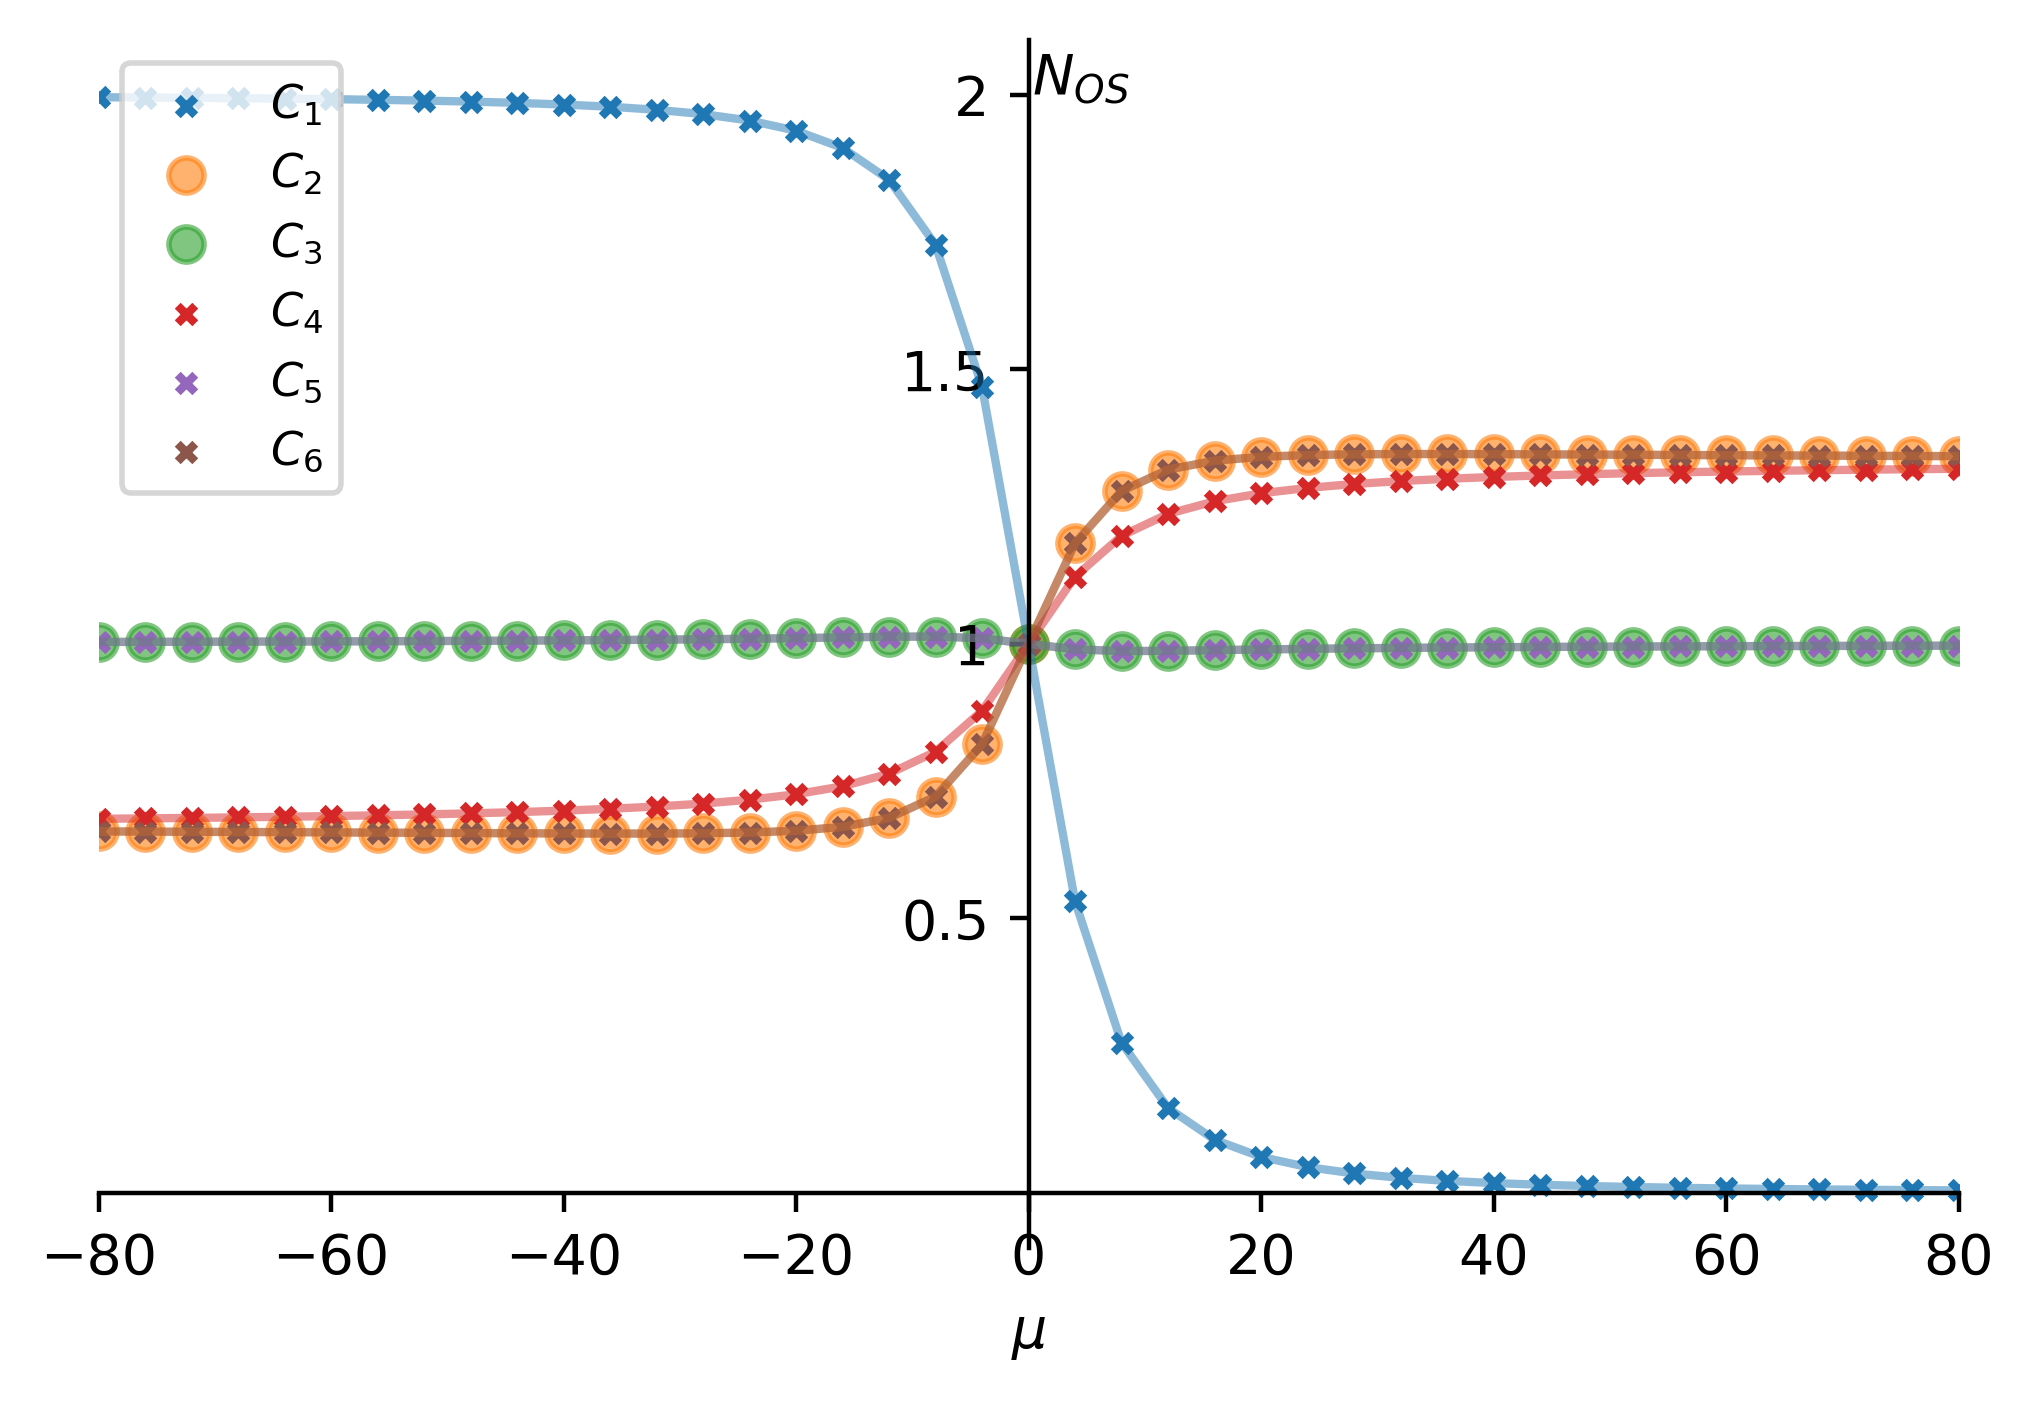
\includegraphics[width=\linewidth]
        {chemical-potential-on-1-carbon-electronpopulation-better.png}
        \caption{Electron population on each carbon atom in function of the applied chemical potential on $C_1$}
        \label{chemical-potential-on-1-carbon-electronpopulation}
    \end{figure}
  \end{center}

  When the interaction between $C_1$ and $C_6$ is decreased to the limit of zero with the help of $\hat{N}_{\beta}^{16}$ the system approximates a transition from benzene to hexa-1,3,5-triene. In both limits, $N_1$ = 0 or 2, the electron distribution for benzene and hexa-1,3,5-triene is found to be the same (\cref{pericyclic-electronpopulation}). But when $N_1$ increases to two or decreases to zero variations occur. In the situation of benzene $C_2$ and $C_6$ will have the same curve but when the interaction is lowered the electron population on $C_2$ will change more with changing the chemical potential than $C_6$. This is because there are fewer carbons atoms between $C_1$ and $C_2$ than between $C_1$ and $C_6$. This shows that a chemical potential will have a different influence on the carbons when interaction is decreased because the carbon atoms will all have different chemical environments due to the linear system.   


  The mutual information does not change with changing interaction when the electron population on $N_1$ is zero(\cref{pericyclic-correlation} $N_1$ = 0). More change is seen when $N_1$ equals one, it can be seen that in the approximation of hexa-1,3,5-triene an alternated structure appears in the entanglement between adjacent carbon atoms. 
  $I_{\Omega_1:\Omega_3}$ and $I_{\Omega_1:\Omega_5}$ are still zero in the approximation of hexa-1,3,5-triene but correlation between $C_1$ and the other carbon atoms decreases the further away they are. $I_{\Omega_2:\Omega_5}$ is also zero too which indicates that a change of the electron population on one of these atoms in the $\pi$-system will do not have a significant influence on the electron population of the other.
  
  The result is that there is an alternated structure formed in the mutual information of hexa-1,3,5-triene. This means that the introduction of a chemical potential has a different influence on the electron distribution in benzene than hexa-1,3,5-triene. The change in electron population at a site, correlated with $C_1$, is greater when fewer bonds separate them.

\subsection{A change of the chemical potential of one site gives insight into the reactivity of simple reagents of a Diels-Alder reaction}

The reagents of another ring closing/opening phenomenon, Diels-Alder, can be proxied in the H$\ddot{\text{u}}$ckel model by decreasing two $\beta$ parameters with $\hat{N}_{\beta}^{ij}$ to the zero interaction limit which can be seen as splitting the benzene system to a butadiene and an ethene system.

The effect of an adjacent external potential on one of the two lowered $\beta$ can be compared to the situation where the external potential is not adjacent. This comparison is illustrated by considering a carbon atom within a butadiene molecule, where the altering potential places it alternatively as an outer or inner carbon atom.

In the case where $N_1$ drops continuously to zero, the electrons only move to site 4 and 6 when $\beta_{12}$ and  $\beta_{34}$  become zero (\cref{Diels-alder-1-electronpopulation}). In the case where $\beta_{23}$ and  $\beta_{45}$ become zero, the electrons only move to site 2 when $N_1$ is zero (\cref{Diels-alder-2-electronpopulation}).

We observe a similar configuration to one butadiene and one ethene molecule when we look to the mutual information in both situations when the interactions are set to zero but $N_1$=1 (\cref{Diels-alder-1-correlation} and \cref{Diels-alder-2-correlation}). When we look to the approximate butadiene system where $C_1$ is an outer carbon atom, we see that the entanglement between $C_1$ and the other atoms have gone to zero when we reduce $N_1$ to zero which yields in three carbon atoms that are still entangled (\cref{Diels-alder-1-correlation}). $C_6$ is the most correlated with $C_1$ and will get the most electrons but is not isolated. When $C_1$ is an inner carbon atom, $C_2$ is the most entangled with $C_1$ but will become isolated when the electron population decreases to zero on $C_1$ (\cref{Diels-alder-2-correlation}).

This tells us that the place of a chemical potential applied in the alternated $\pi$-system of butadiene will have a major influence on the change in electron population and entanglement.

Such a behavior can also be seen in the substituted butadienes. In a Diels-Alder reaction there is a diene and a dienophile. When these are substituted with different groups the selectivity of the reaction can be influenced. An electron-withdrawing group and electron-donating group will have different regioselectivity because a change of electron distribution, similarly to what is described in HMO. The change of the potential of a carbon can be seen equivalent to a substitution on that carbon. An electron-withdrawing group will draw electrons from the system and when the potential on the carbon is stabilizing the same effect occur. The same is true for electron-donating groups and a destabilizing potential. The thinking can also be used for an aromatic substitution on a substituted benzene. The substituted groups can also be presented here by a change in a potential.

We must consider that although a methoxy group, for instance, is mesomeric electron-donating group, our current approach fails to acknowledge its inductive electron-withdrawing effect on the system. Nevertheless, our approach offers valuable insights into the reactivity of the $\pi$-system. Therefore, we suggest a model where substituted conjugated hydrocarbon compounds are examined by introducing a chemical potential in HMO. While deviations from reality may occur as we move away from benzene, the H$\ddot{\text{u}}$ckel model remains a useful tool for obtaining understanding of molecular behavior.

\section{Conclusions}
We showed how entanglement patterns of the $\pi$ system change when interactions are lowered to zero while a chemical potential is applied to set the electron population on a carbon at a specific value. This was done to approximate the effect on the conjugated $\pi$ system of introducing a hetero atom. While this study does not take the substituted groups that play a role in the Diels-Alder reaction explicitly into account, the analysis show that a chemical potential can be seen as substituting that carbon atom with an electron-donating or electron-withdrawing group. Further exploration of the mutual information is needed to see what the capabilities are to get more insight into the behavior of the conjugated $\pi$-system. On the other hand, if we move beyond the benzene system, the same analysis could be conducted using Restricted Hartree-Fock (RHF) theory to achieve more accurate results.
\newline
\newline
\newline
\newline
\newline
\newline
\newline
\newline
\newline
\newline
\newline
\newline
\newline
\newline
\newline
\newline
\newline
\newline
\newline
\newline
\newline
\newline

%%%END OF MAIN TEXT%%%

%The \balance command can be used to balance the columns on the final page if desired. It should be placed anywhere within the first column of the last page.



%If notes are included in your references you can change the title from 'References' to 'Notes and references' using the following command:
%\renewcommand\refname{Notes and references}

%%%REFERENCES%%%
\bibliography{research-outline} %You need to replace "rsc" on this line with the name of your .bib file
\bibliographystyle{aip} %the AIP's .bst file
\begin{center}
  \begin{figure*}[!htbp]
      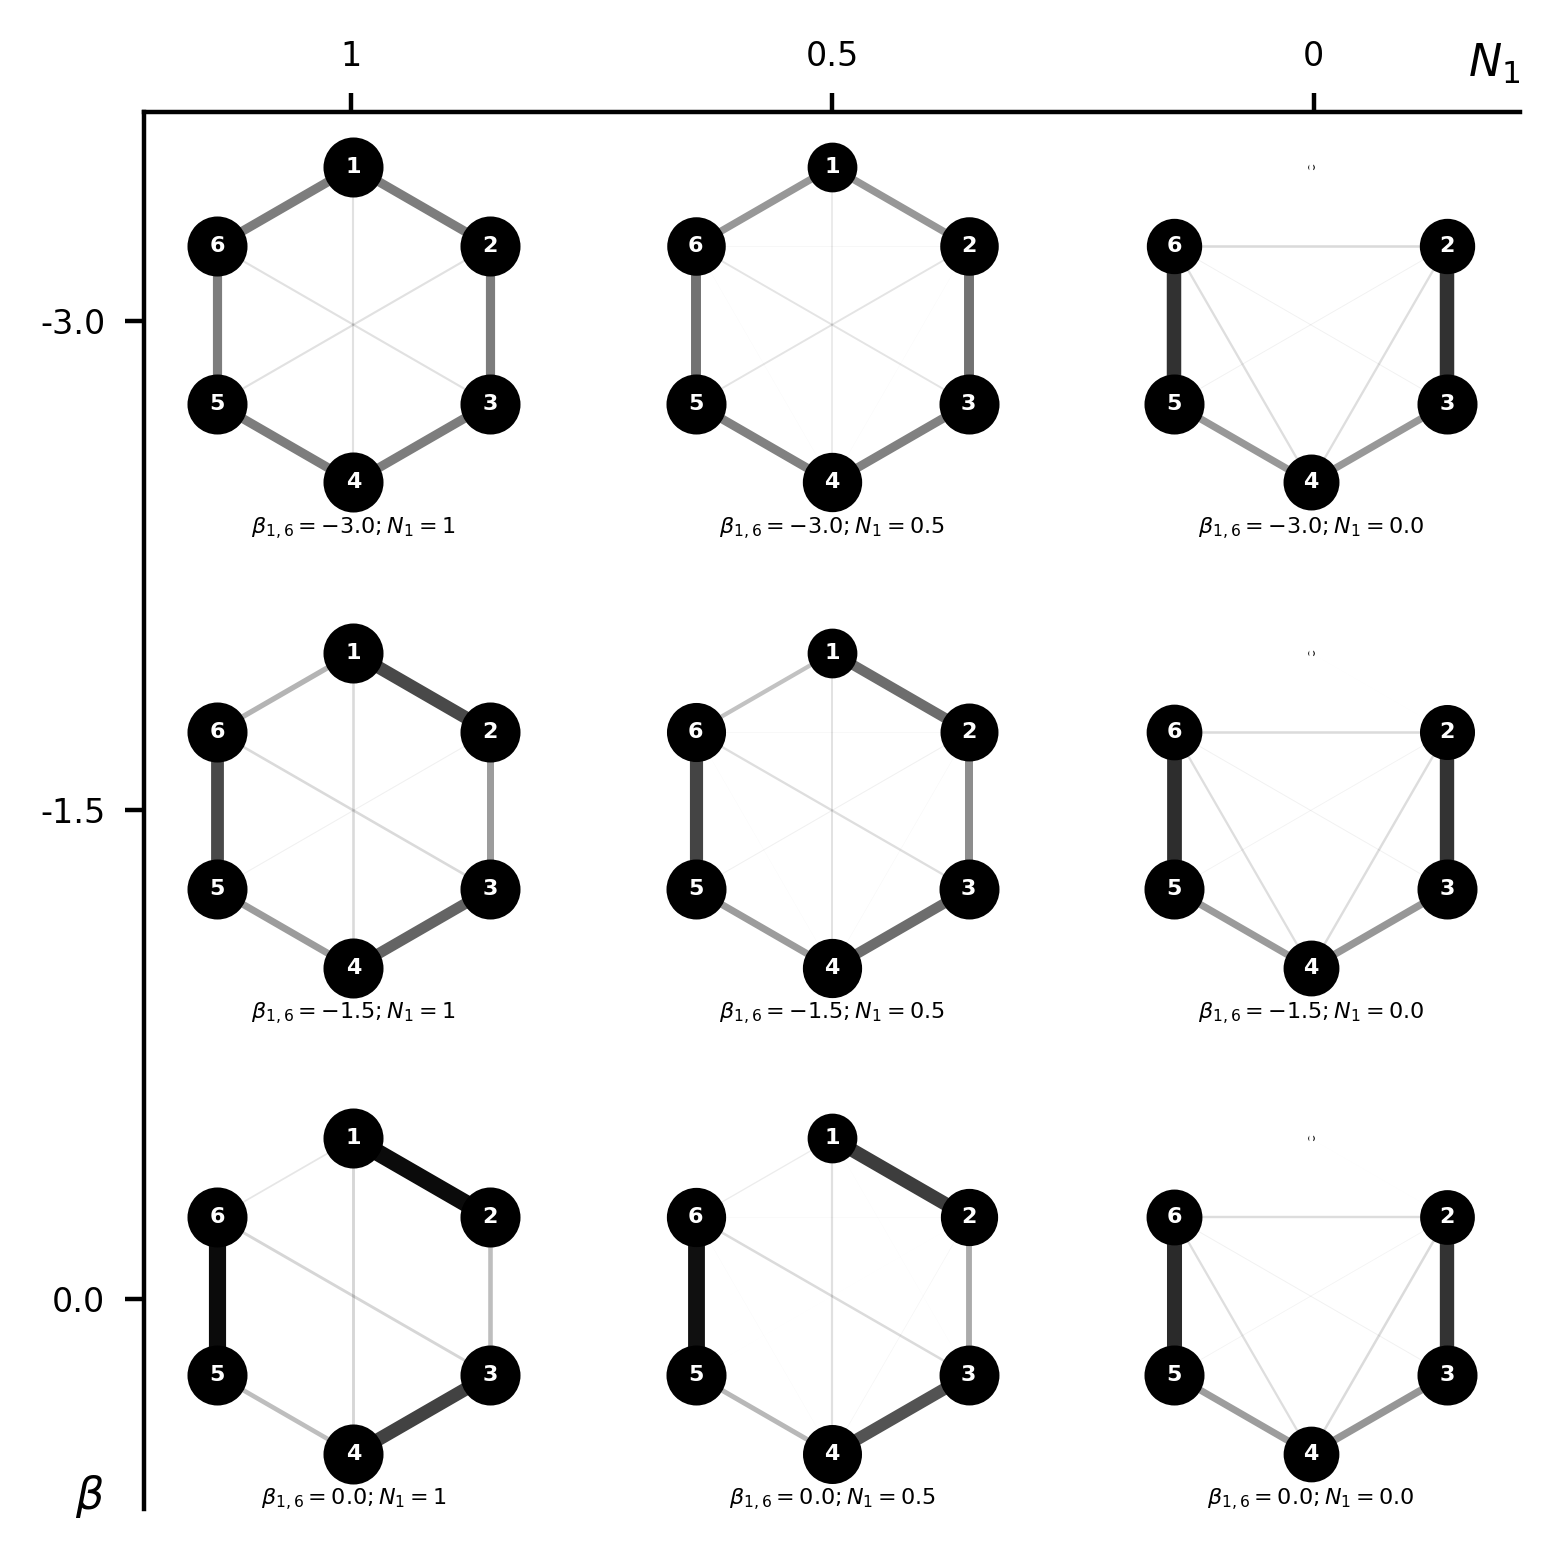
\includegraphics[width=\textwidth]{Benzene-correlation-potential-and-one-adjacent-beta.png}
      \caption{Mutual information when varying $N_1$ and different $\beta_{16}$ = $\beta_{61}$ where $\beta_{16}$  = -3 represents benzene and $\beta_{16}$ = 0 Hexa-1,3,5-triene. The thickness and opacity of the line represents the magnitude of the mutual information between two carbons atoms, and the size of the nodes represents the entanglement entropy of each individual carbon atoms.}
      \label{pericyclic-correlation}
  \end{figure*}
\end{center}

\begin{center}
  \begin{figure*}[!htbp]
      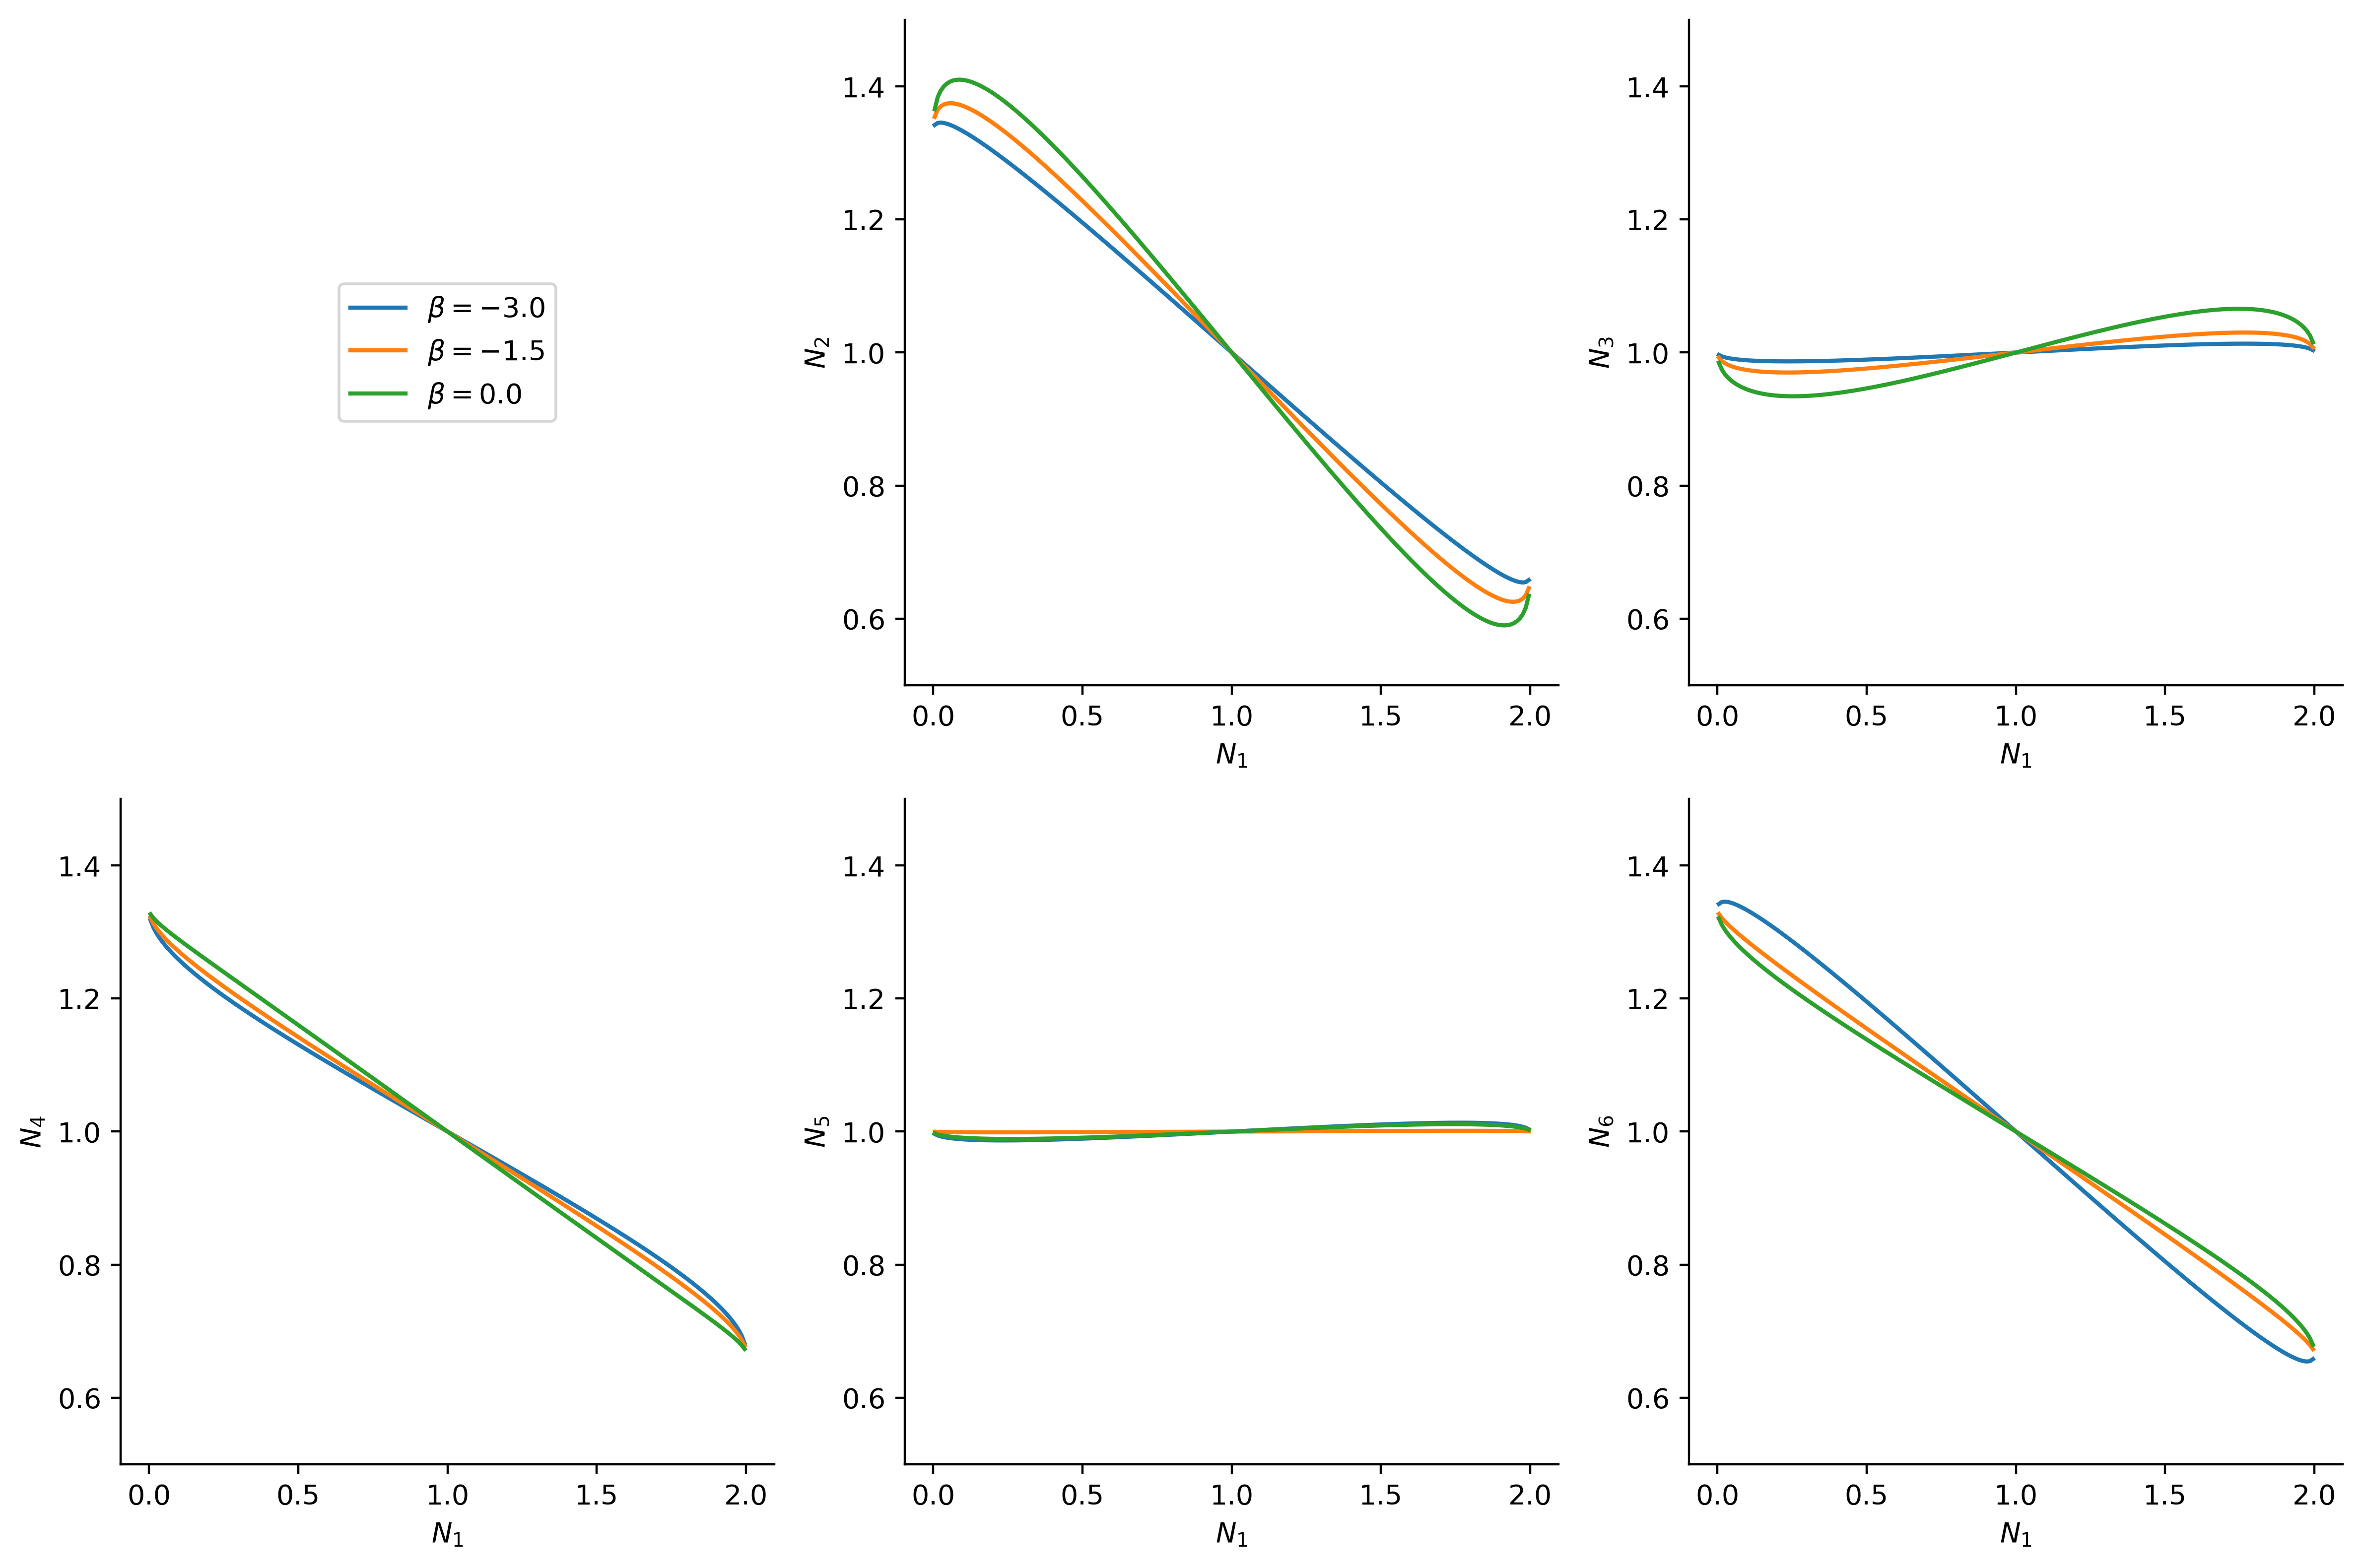
\includegraphics[width=\textwidth]{Benzene-electronpopulation-on-atoms-potential-and-one-adjacent-beta.png}
      \caption{Electron population on each carbon atom when varying the electron population on $C_1$ for different $\beta_{16}$ = $\beta_{61}$where $\beta_{16}$ = -3 represents benzene and $\beta_{16}$ = 0 Hexa-1,3,5-triene}
      \label{pericyclic-electronpopulation}
  \end{figure*}
\end{center}

\begin{center}
  \begin{figure*}[!htbp]
      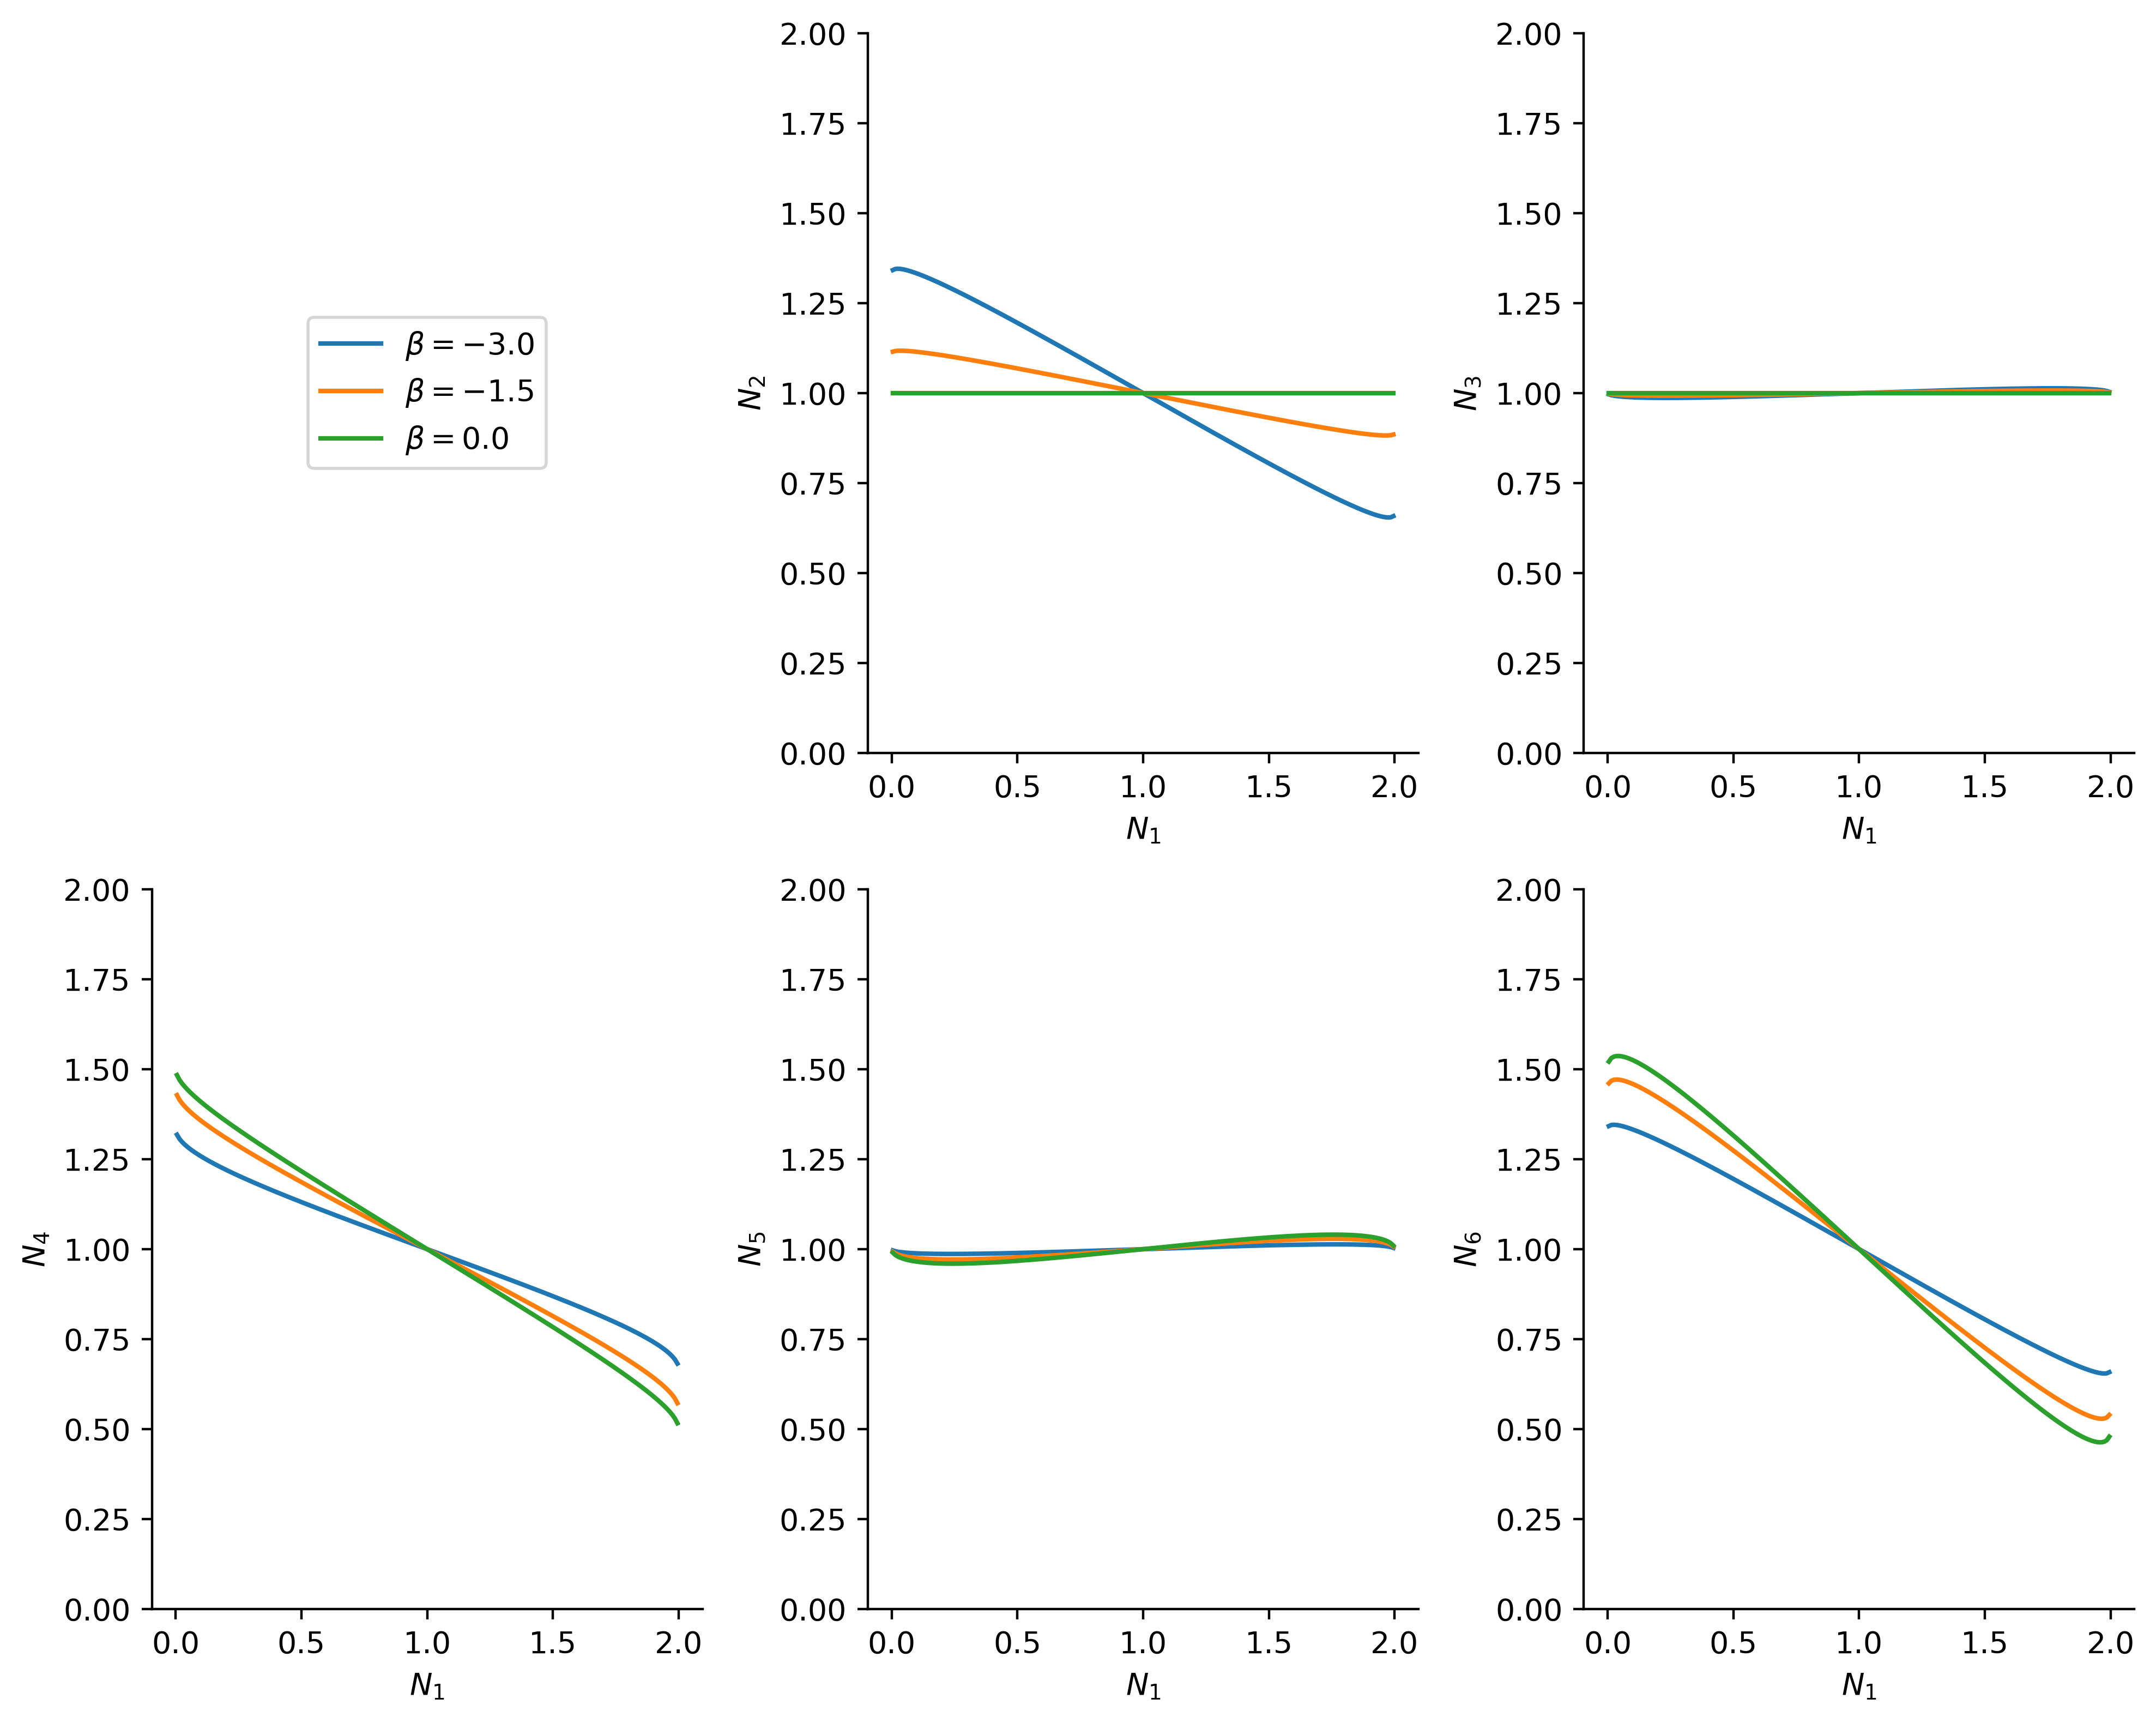
\includegraphics[width=\textwidth]{Benzene-electronpopulation-on-atoms-potential-and-two-betas-to-zero-adjacent.png}
      \caption{Electron population on each carbon atom when varying the electron population on $C_1$ and different $\beta$ between $C_1$-$C_2$ and $C_3$-$C_4$.}
      \label{Diels-alder-1-electronpopulation}
  \end{figure*}
\end{center}

\begin{center}
  \begin{figure*}[!htbp]
      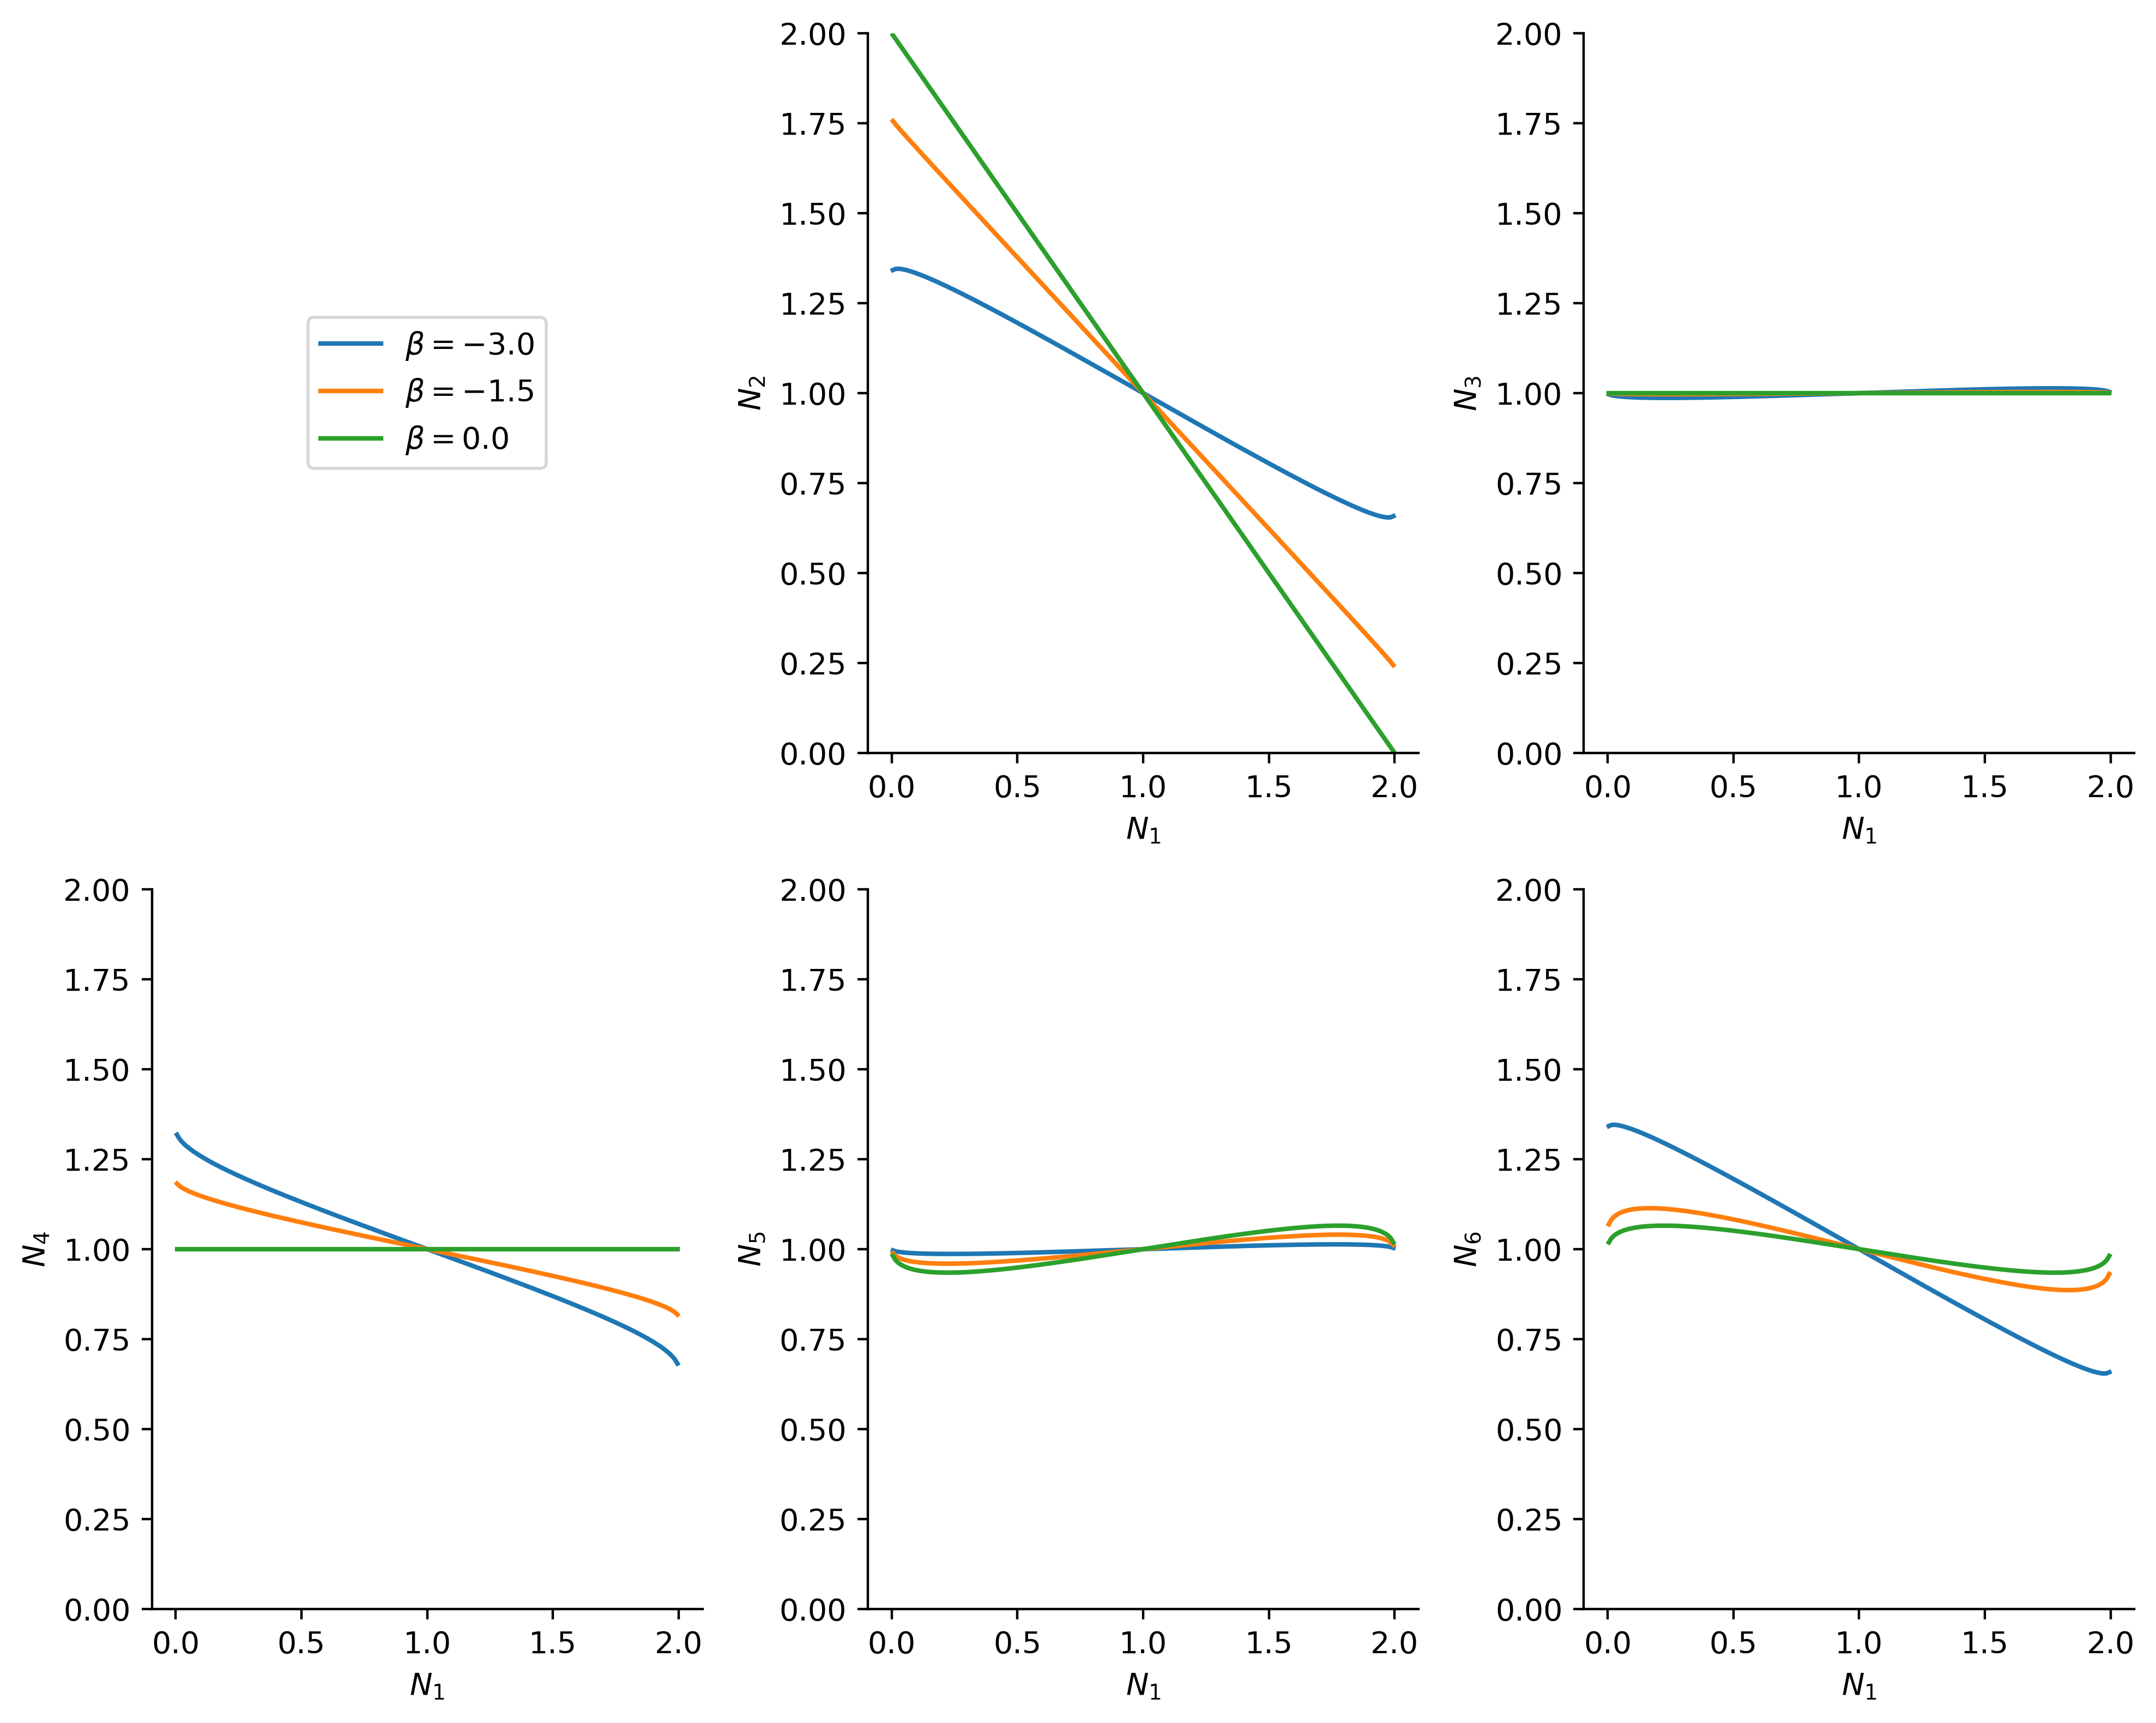
\includegraphics[width=\textwidth]{Benzene-electronpopulation-on-atoms-potential-and-two-betas-to-zero-not-adjacent.png}
      \caption{Electron population on each carbon atom when varying the electron population on $C_1$ and different $\beta$ between $C_2$-$C_3$ and $C_4$-$C_5$.}
      \label{Diels-alder-2-electronpopulation}
  \end{figure*}
\end{center}

\begin{center}
  \begin{figure*}[!htbp]
      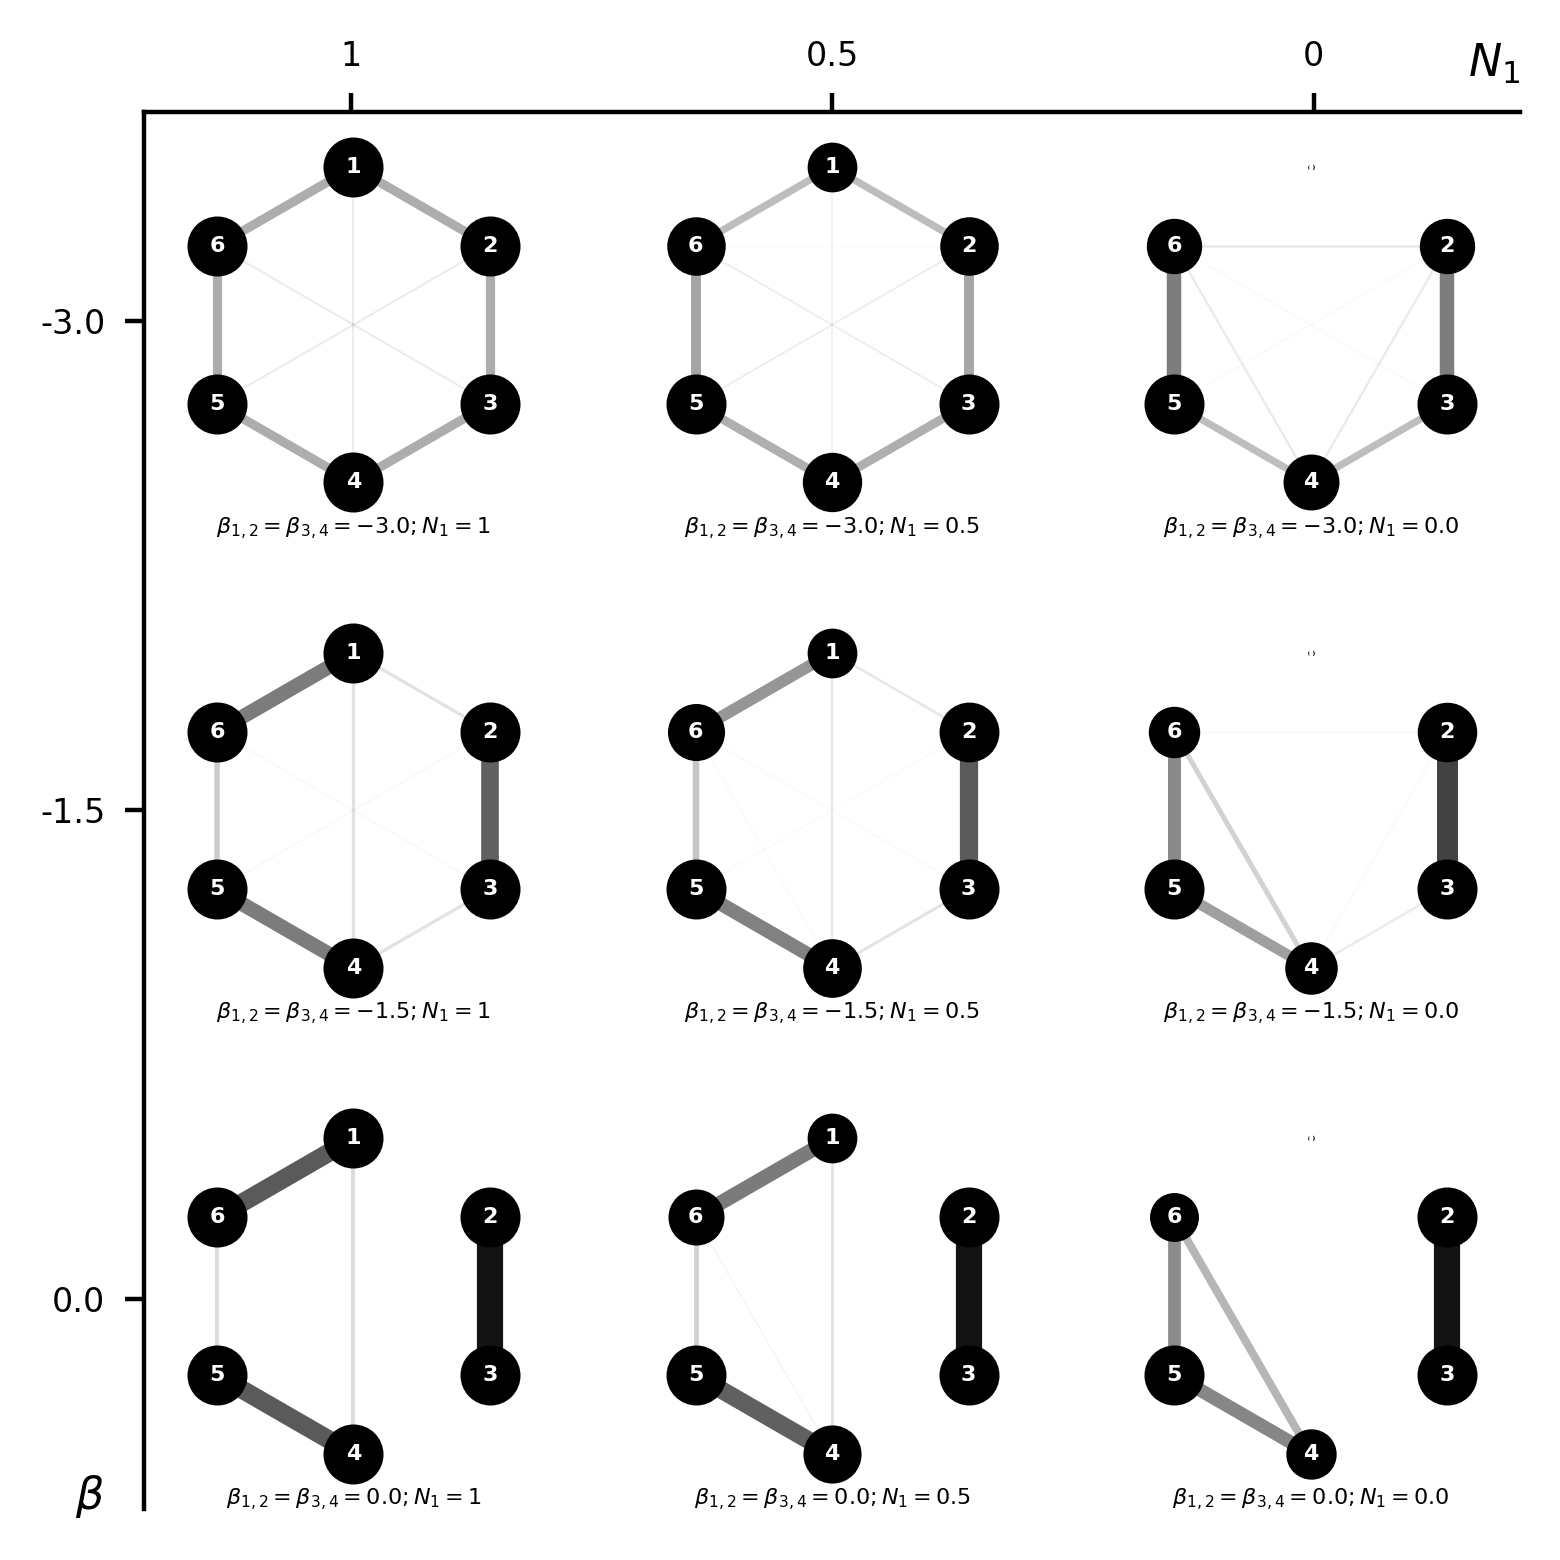
\includegraphics[width=\textwidth]{Benzene-correlation-potential-and-two-betas-to-zero-adjacent.png}
      \caption{Mutual information when varying the electron population on $C_1$ and different $\beta$ between $C_1$-$C_2$ and $C_3$-$C_4$.  The thickness and opacity of the line represents the magnitude of the mutual information between two carbons atoms, and the size of the nodes represents the entanglement entropy of each individual carbon atoms.}
      \label{Diels-alder-1-correlation}
  \end{figure*}
\end{center}

\begin{center}
  \begin{figure*}[!htbp]
      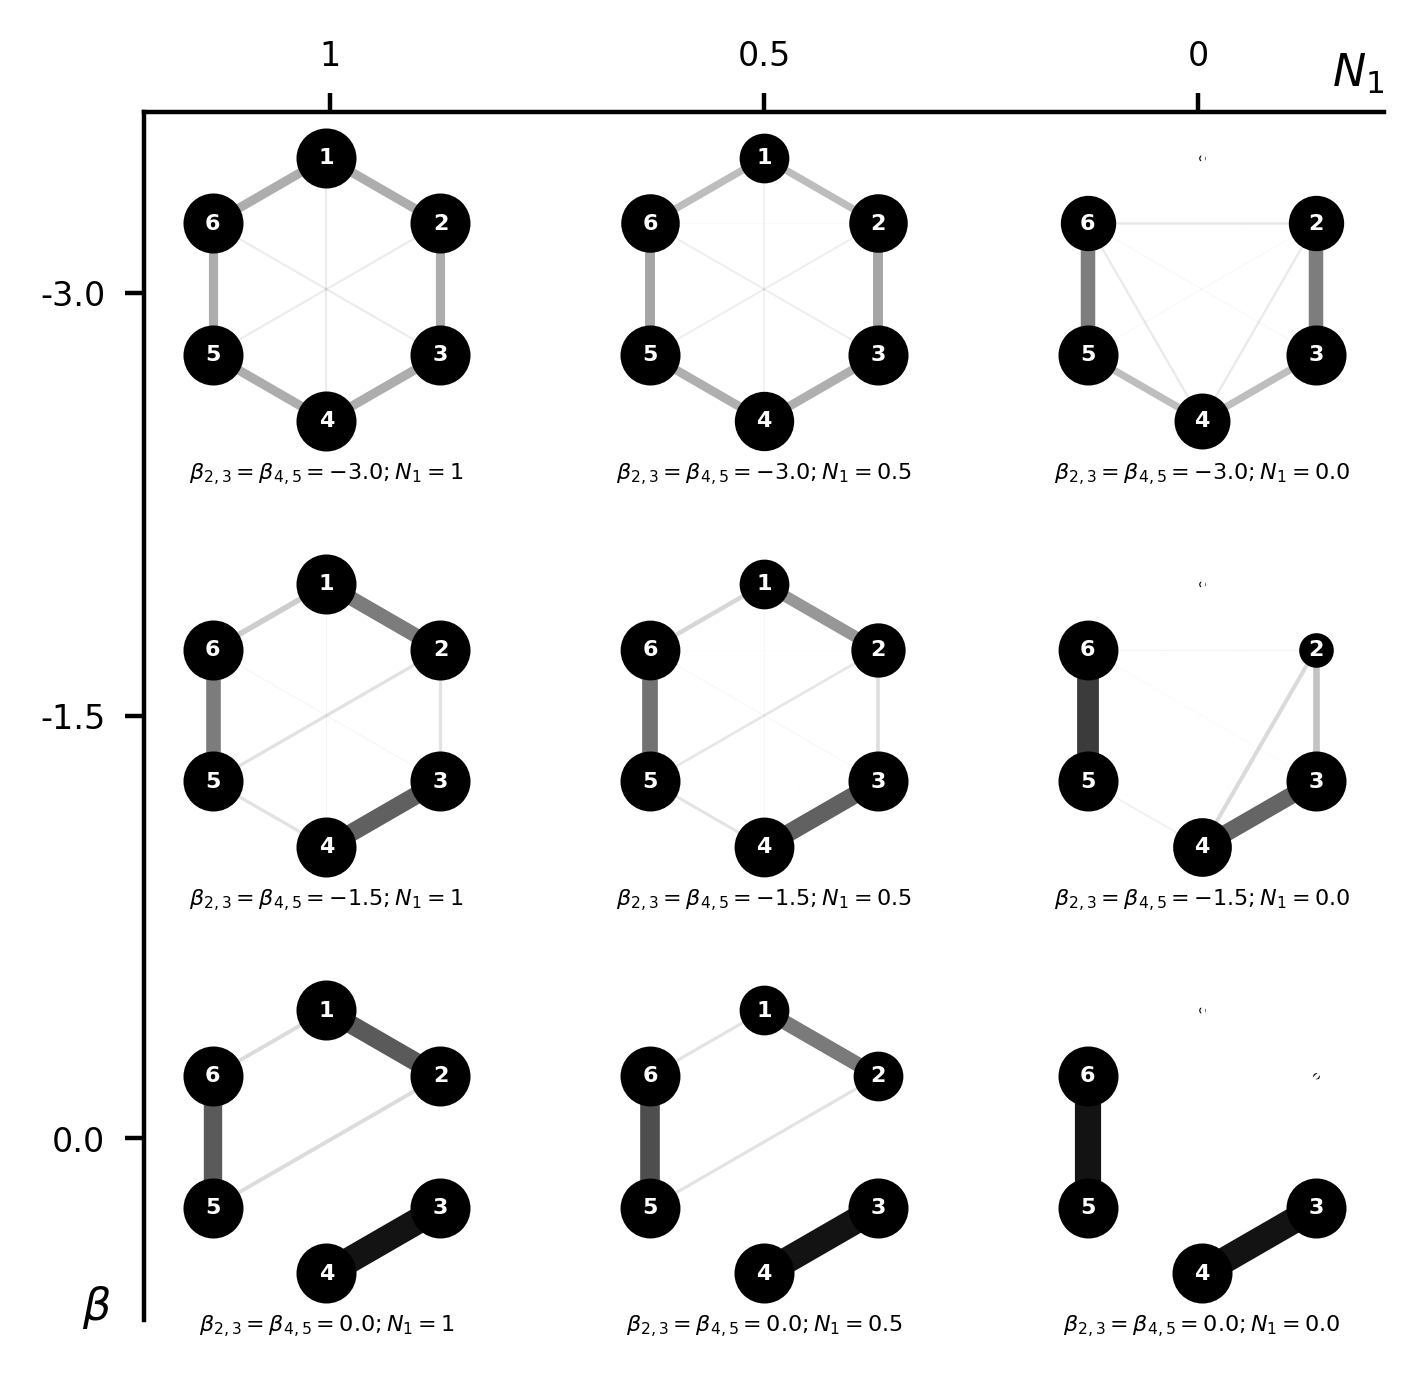
\includegraphics[width=\textwidth]{Benzene-correlation-potential-and-two-betas-to-zero-not-adjacent.png}
      \caption{Mutual information when varying the electron population on $C_1$ and different $\beta$ between $C_2$-$C_3$ and $C_4$-$C_5$.  The thickness and opacity of the line represents the magnitude of the mutual information between two carbons atoms, and the size of the nodes represents the entanglement entropy of each individual carbon atoms.}
      \label{Diels-alder-2-correlation}
  \end{figure*}
\end{center}
 
\newpage
\appendix 
\section{Comparing HMO with RHF for the $\pi$-system of benzene} \label{sec:HMO vs RHF for benzene}
\begin{center}
  \begin{figure}[H]
      \includegraphics[width=\linewidth]{MO-Benzene-hückel.png}
      \caption{H$\ddot{\text{u}}$ckel:6 MO's of $\pi$-system of benzene molecule in 2$p_z$-basis of the carbon atoms}
      \label{fig:MO-Benzene-hückel}
  \end{figure}
\end{center}
\begin{center}
  \begin{figure}[H]
      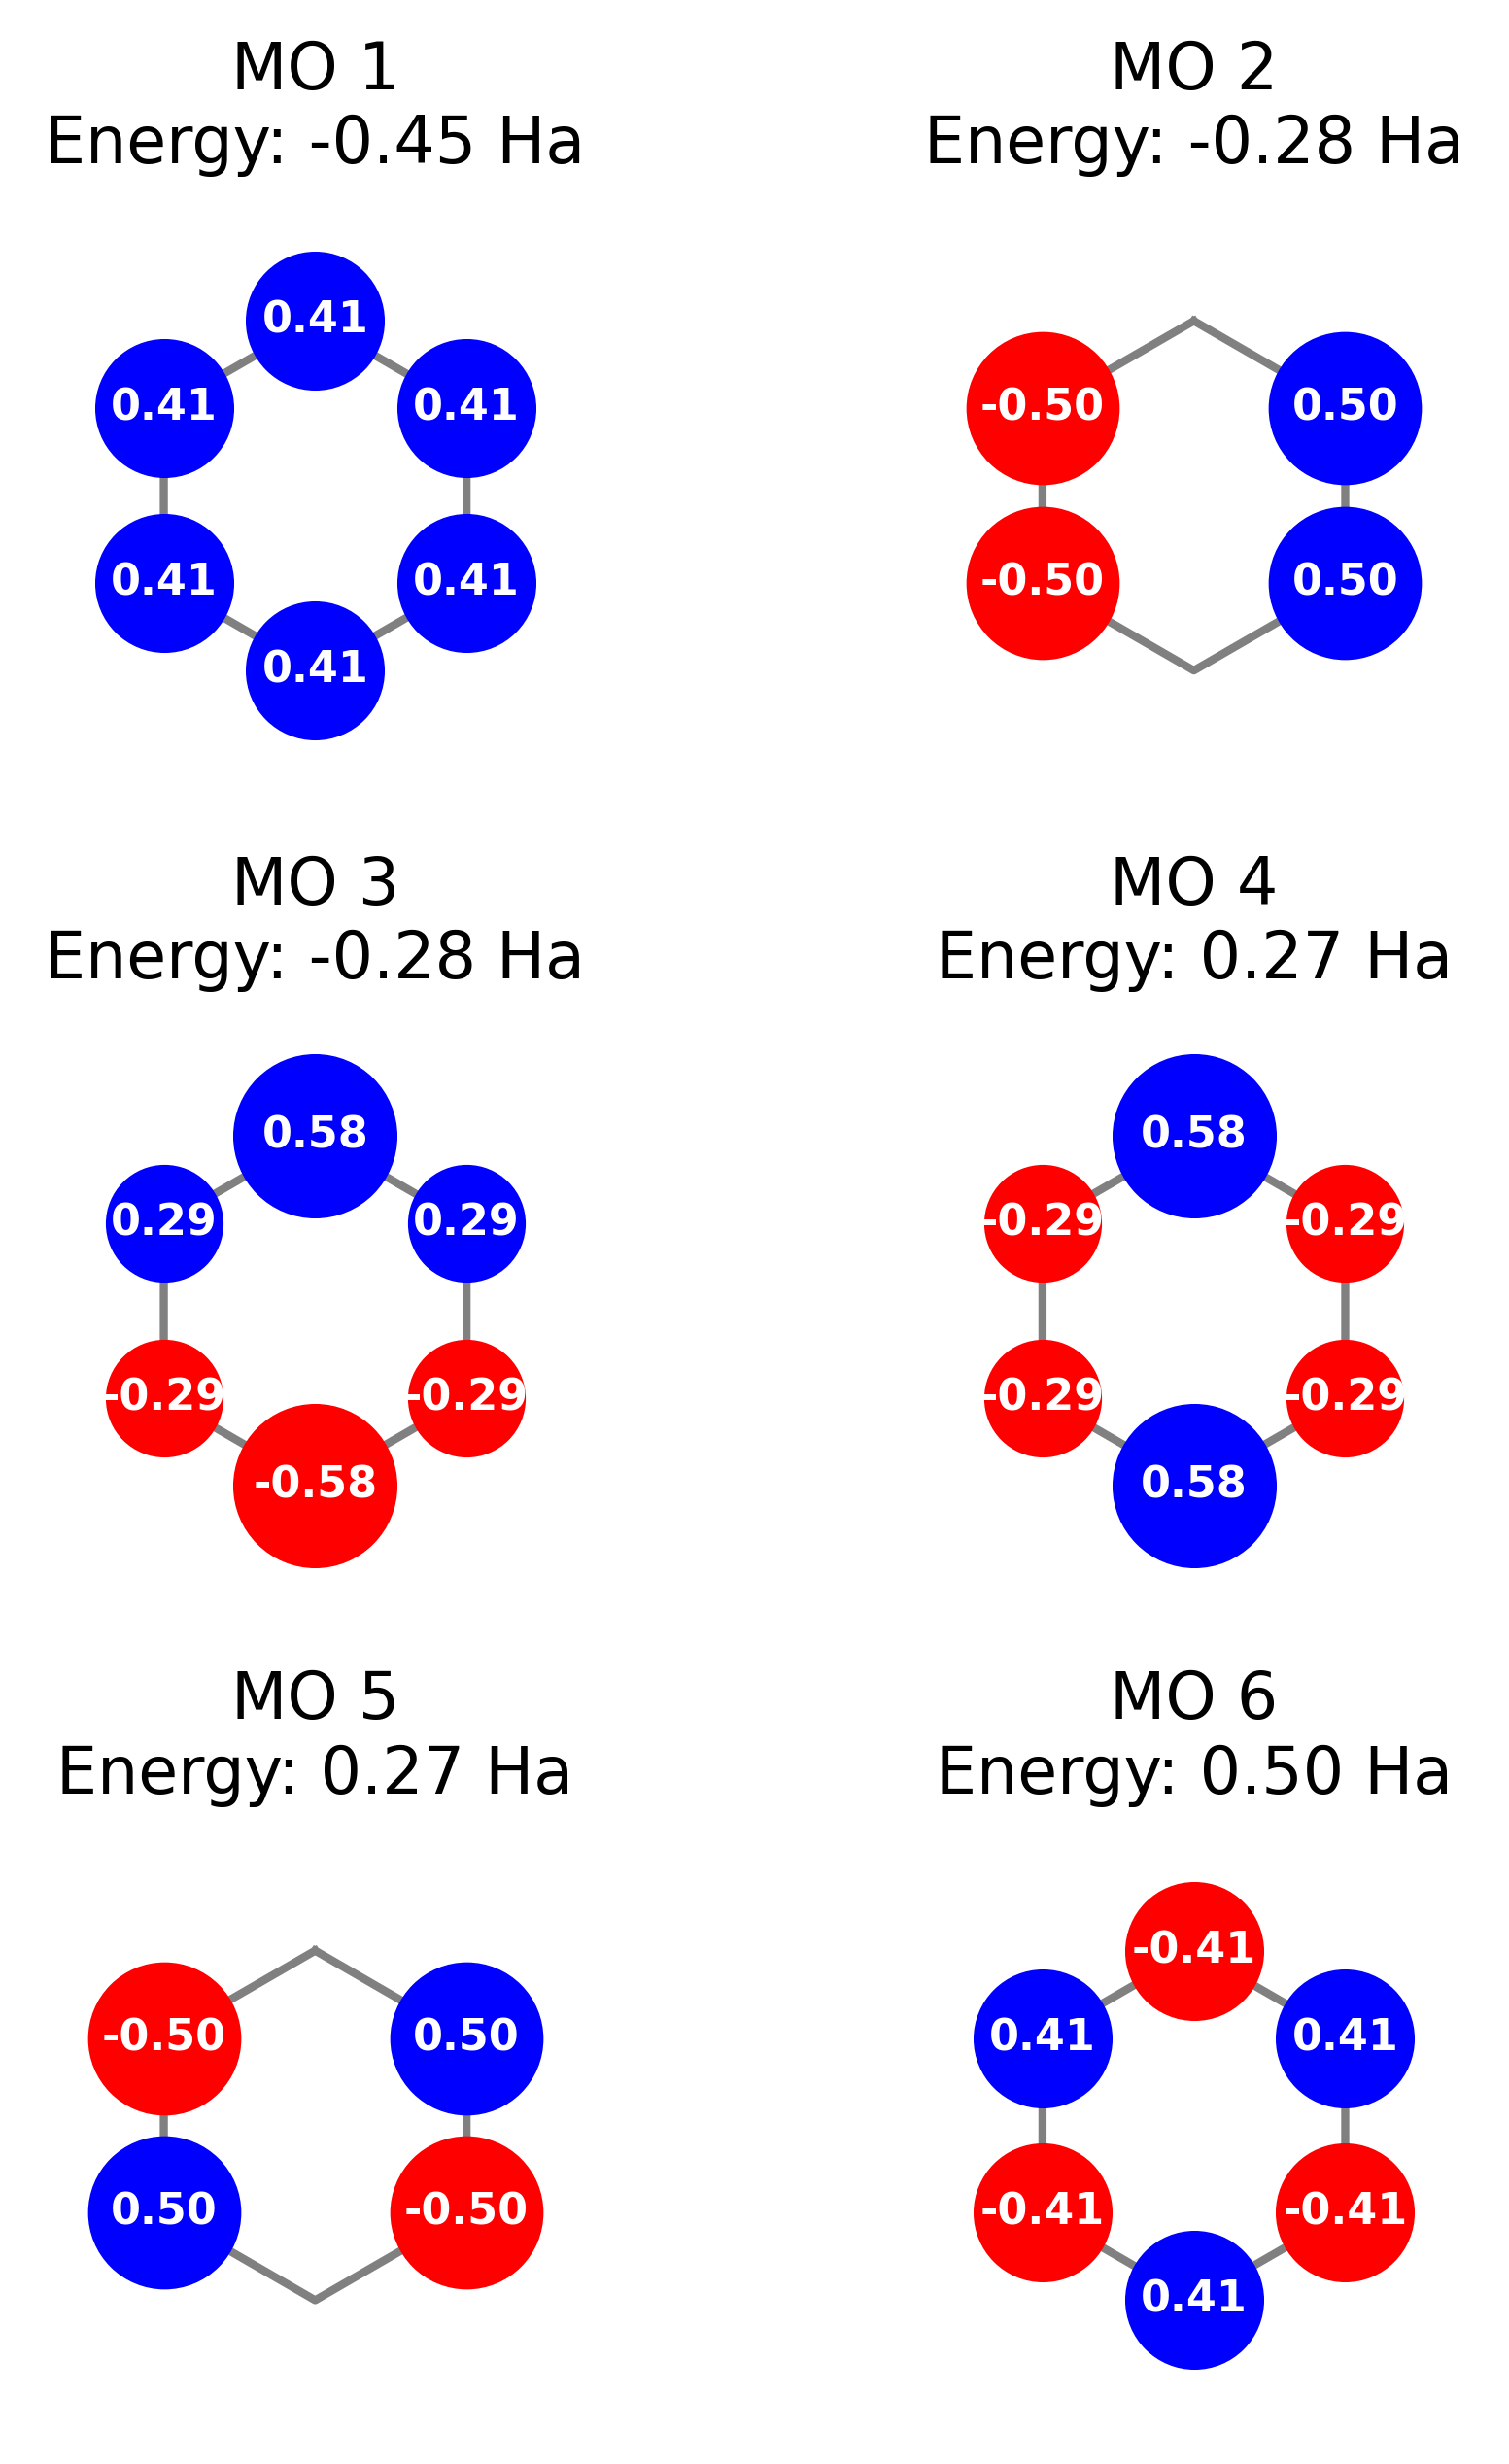
\includegraphics[width=\linewidth]{MO-Benzene-6-rhf-sto-3g.png}
      \caption{RHF: 6 MO's of $\pi$-system of benzene molecule in sto-3g basis where the coefficients of the 2$p_z$ atomic orbitals are plotted on the corresponding carbon atom.}
      \label{fig:MO-Benzene-RHF-6-sto-3g}
  \end{figure}
\end{center}

\end{document}
